\chapter{Testing}\label{ch:testing}
This chapter of the report will detail the testing conducted on the configured AWS services.
This was done to determine the accuracy and efficiency of the configurations made during the deployment process.
The testing was conducted by using Gherkin, a language used to define behaviour and test
cases~\parencite{dos2018automated}.
It is non-technical and is intended to be easily human-readable.
Gherkin uses set keywords for structure and meaning: Given, When, and Then.
An example of this structure can be seen in figure below.

\begin{figure}[!htbp]
    \centering
    \begin{minted}{cucumber}
    Scenario: ...
        Given ...
        When ...
        Then ...
    \end{minted}
    \label{fig:gherkin}
\end{figure}

EC2, S3, CloudFront, RDS, CloudWatch, and CloudTrail were all tested using this approach.
Screenshots are included to illustrate the results of these tests.

\section{Testing EC2}\label{sec:testing-ec2}
\begin{figure}[!htbp]
    \centering
    \begin{minted}{cucumber}
Scenario: Accessing instance through SSH with .pem file private key.
    Given that the EC2 instance is running on AWS and the user has EC2 keypair
    When the user enters the command
    "ssh -i Group4_KeyPair.pem ec2-user@35.169.71.228" in the terminal
    Then the user will be logged into the EC2 instance
    \end{minted}
    \label{fig:accessing-instance-ec2}
\end{figure}

\begin{figure}[!htbp]
    \centering
    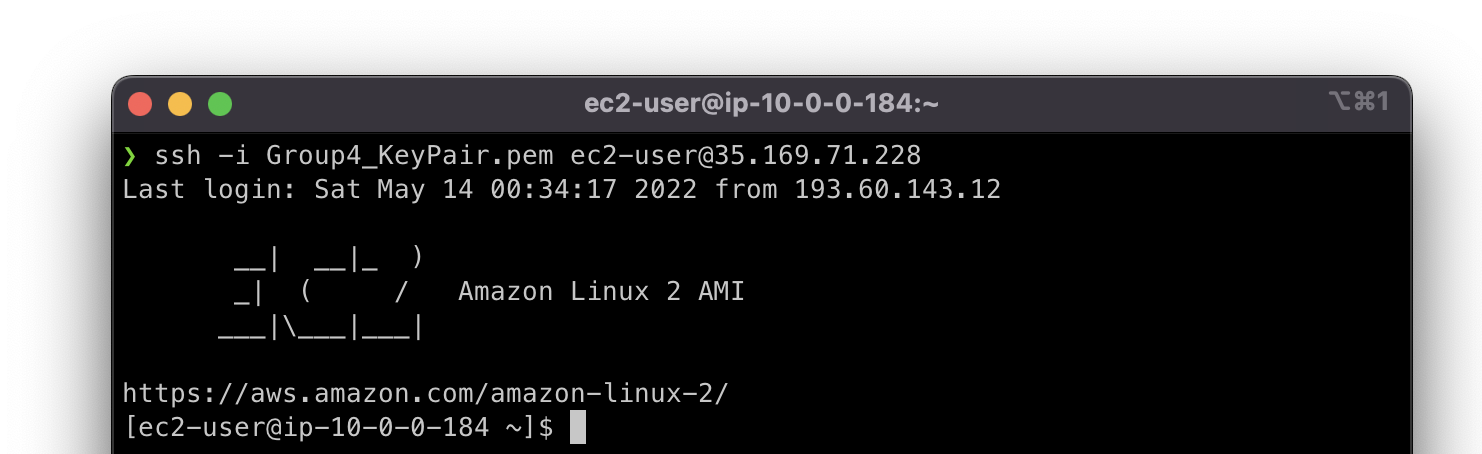
\includegraphics[width=\textwidth]{resources/ec2/ec2-logged-in}
    \label{fig:ec2-test-logged-in}
\end{figure}

\clearpage
\begin{figure}[!htbp]
    \centering
    \begin{minted}{cucumber}
Scenario: Accessing web app through EC2 domain name.
    Given that the web app is running on the EC2 instance
    When the user accesses
    "http://ec2-35-169-71-228.compute-1.amazonaws.com/" in their browser
    Then the web app will be loaded
    \end{minted}
    \label{fig:accessing-web-app-ec2}
\end{figure}

\begin{figure}[!htbp]
    \centering
    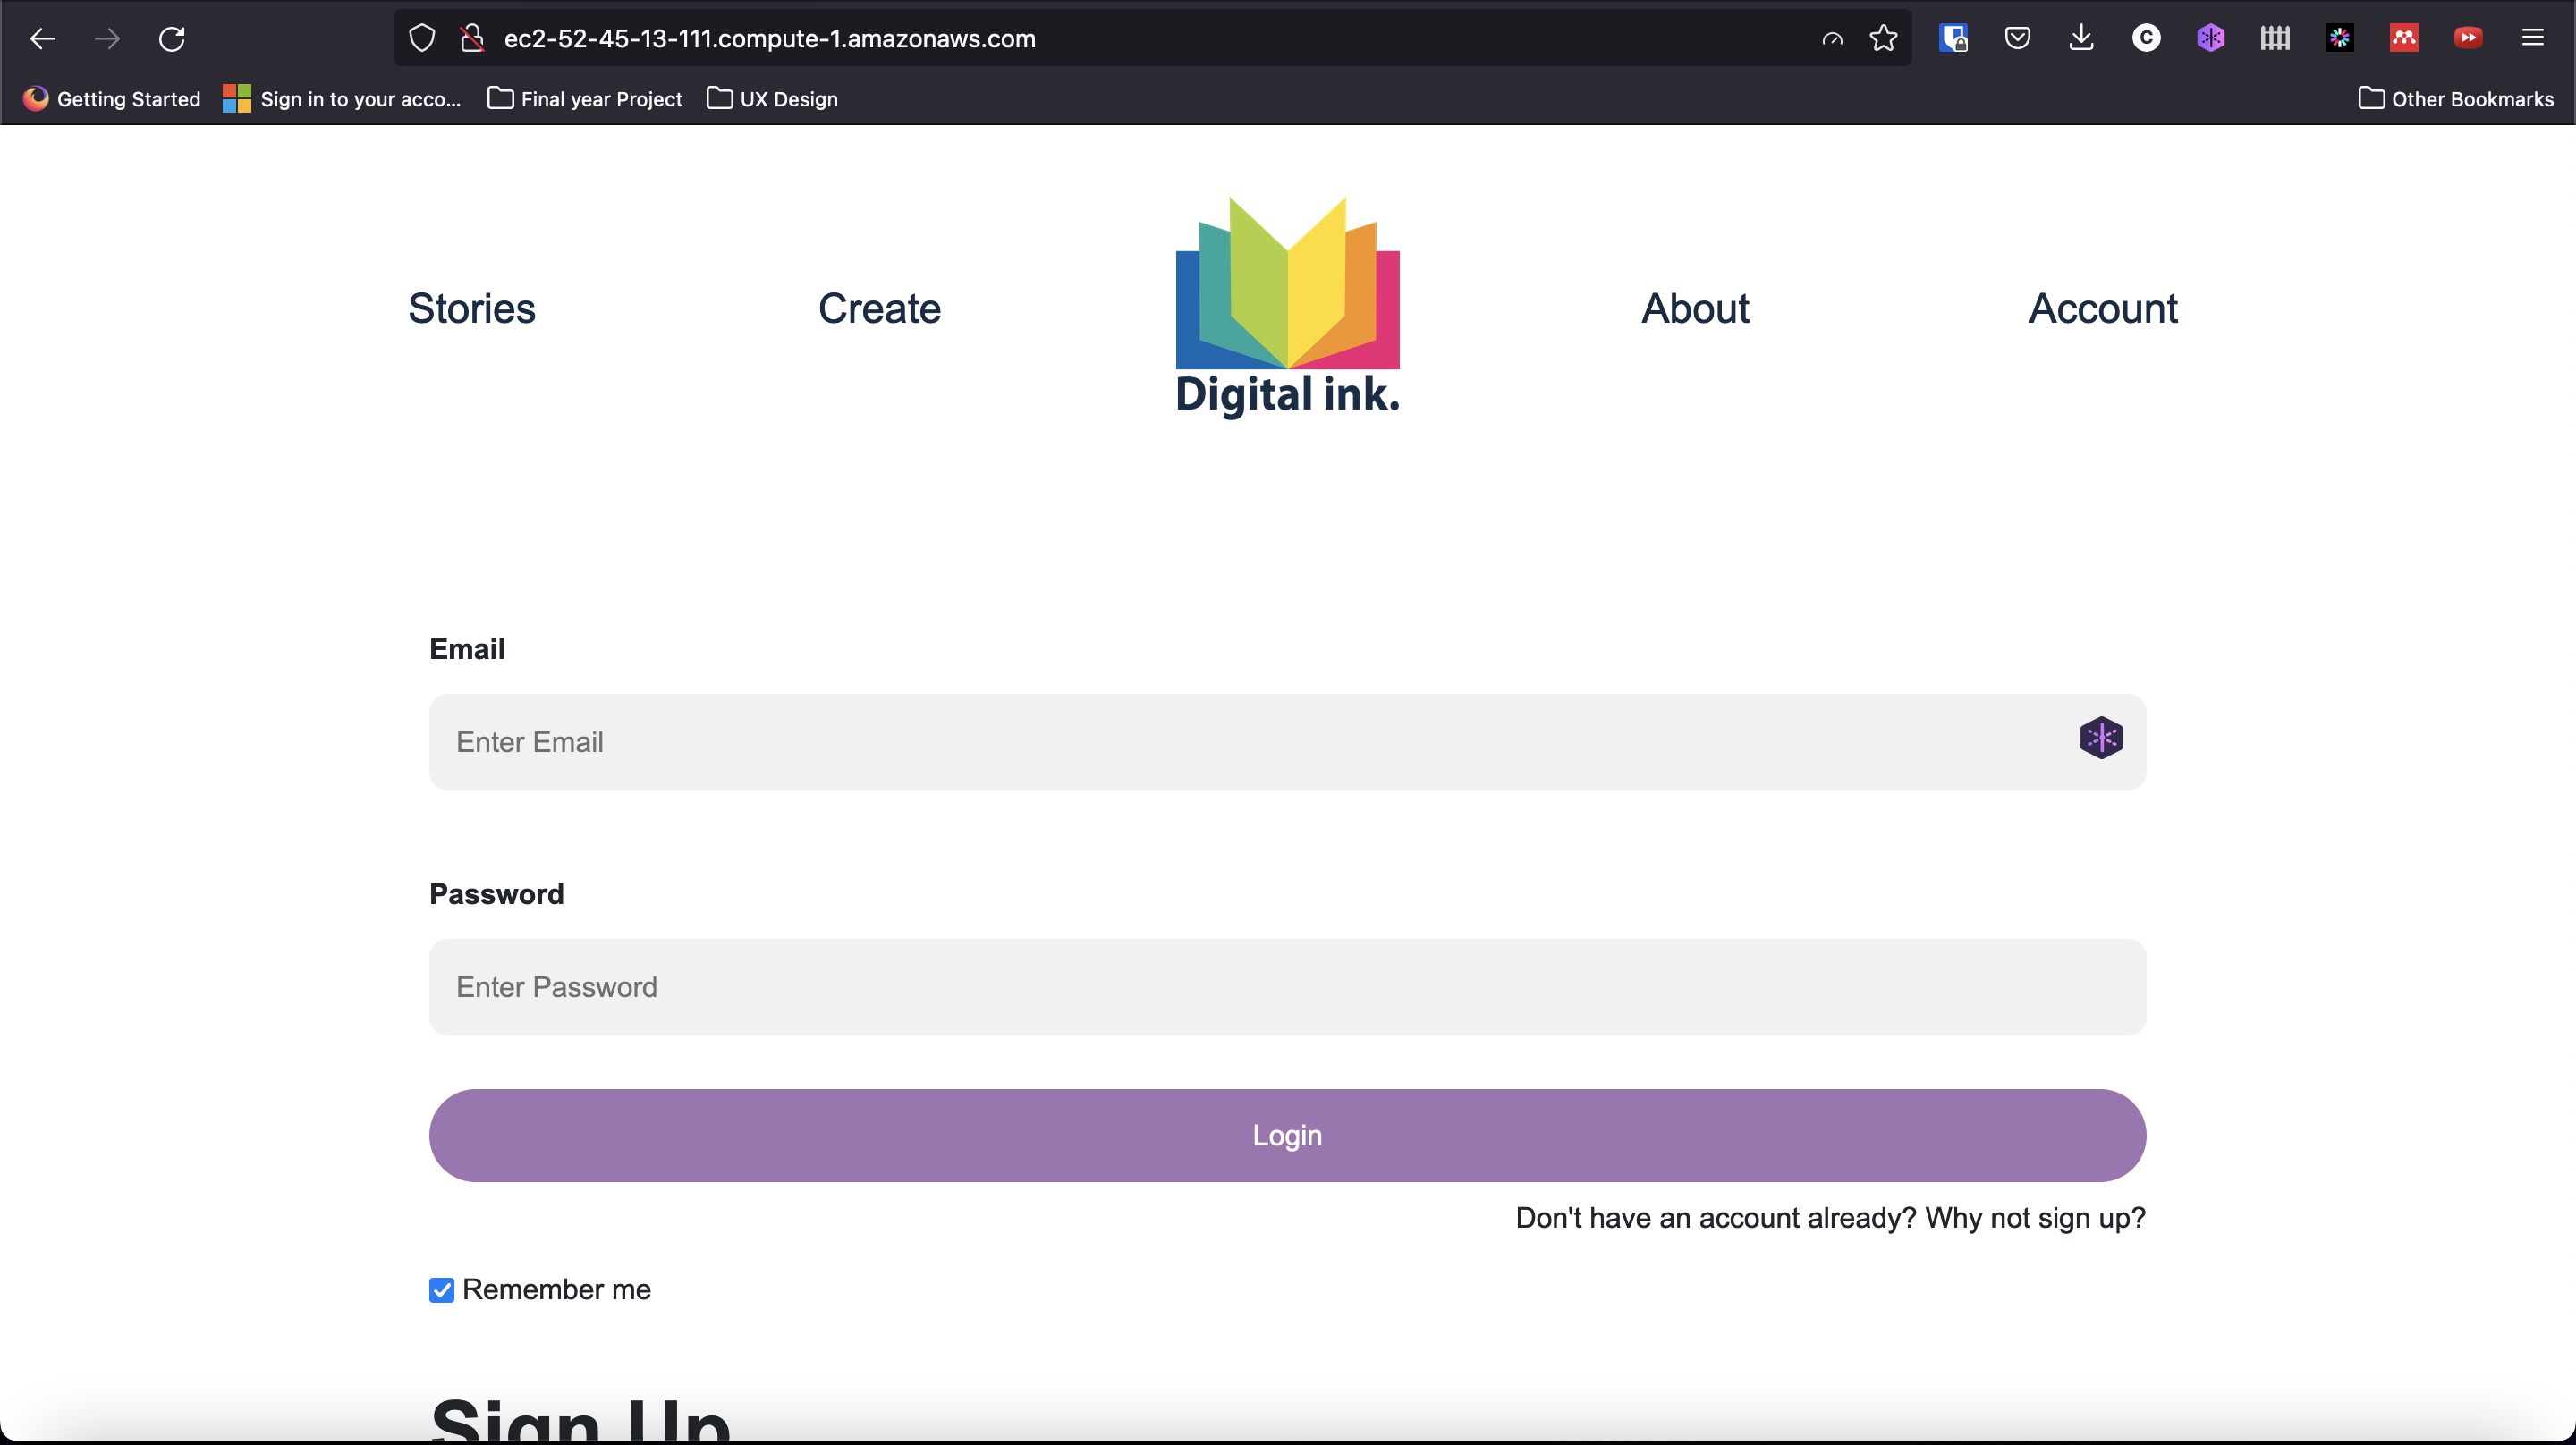
\includegraphics[width=\textwidth]{resources/ec2/digital-ink-ec2}
    \label{fig:ec2-test-digital-ink}
\end{figure}

\clearpage
\section{Testing S3}\label{sec:testing-s3}
\begin{figure}[!htbp]
    \centering
    \begin{minted}{cucumber}
Scenario: Accessing web app image through S3 domain name.
    Given that an image on the web app is in an S3 bucket
    When the user accesses the URL
    "https://group4-digital-ink-s3.s3.amazonaws.com/" followed by the name of the image
    Then the user will see the image displayed from the S3 bucket
    \end{minted}
    \label{fig:accessing-image-s3}
\end{figure}

\begin{figure}[!htbp]
    \centering
    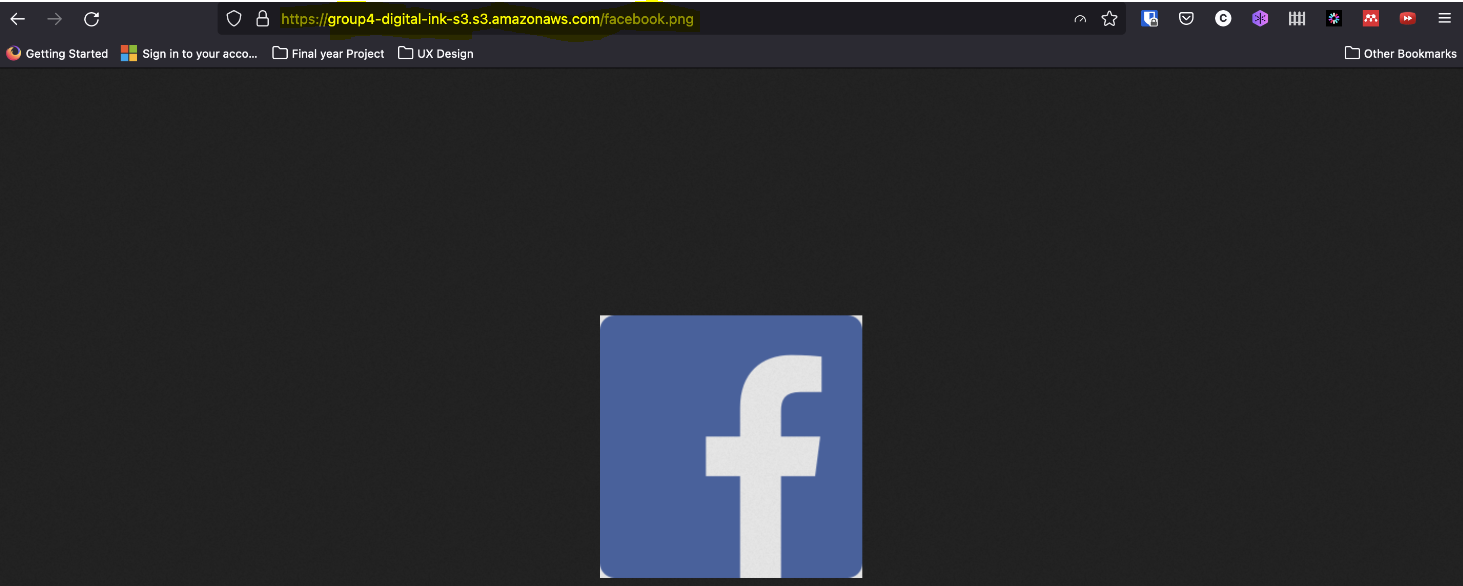
\includegraphics[width=125mm]{resources/s3/s3-image-displayed}
    \label{fig:s3-test-photo}
\end{figure}

\section{Testing CloudFront}\label{sec:testing-cloudfront}
\begin{figure}[!htbp]
    \centering
    \begin{minted}{cucumber}
Scenario: Accessing web app image through CloudFront domain name.
    Given that an image on the web app is in a CloudFront distribution
    When the user accesses the URL
    "https://d1bdkf7iuqj4qy.cloudfront.net/" followed by the name of the image
    Then the user will see the image displayed from the CloudFront distribution
    \end{minted}
    \label{fig:accessing-image-cloudfront}
\end{figure}

\begin{figure}[!htbp]
    \centering
    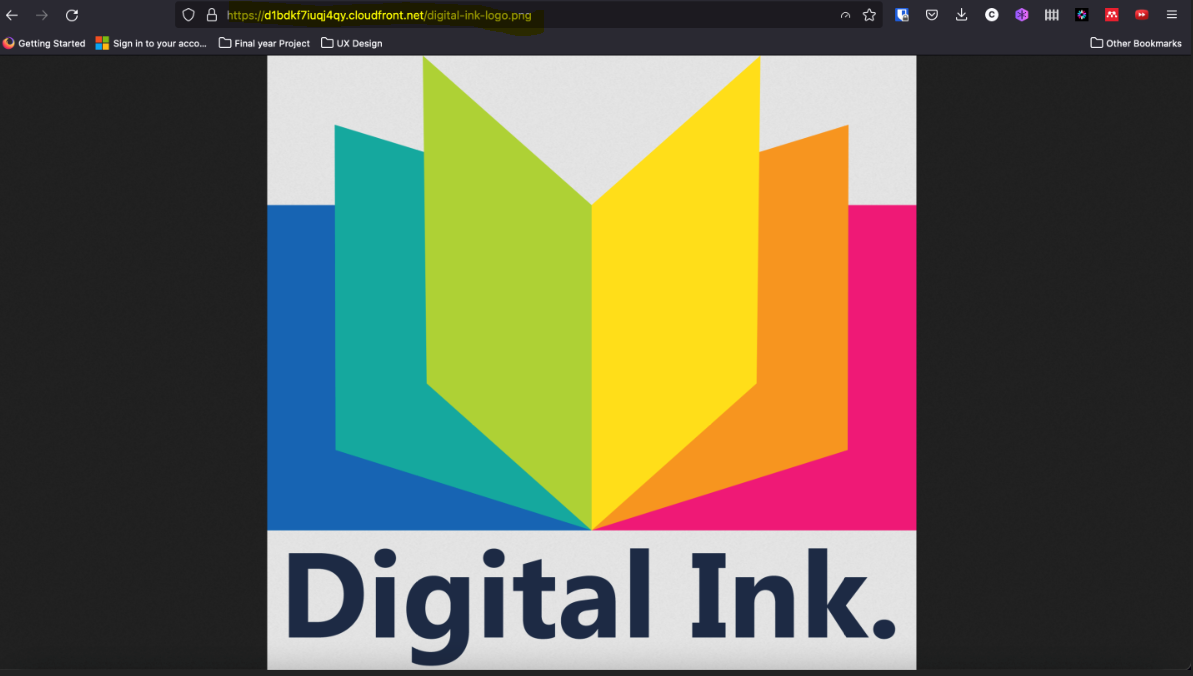
\includegraphics[width=125mm]{resources/cloudfront/cloudfront-website}
    \label{fig:cloudfront-test-photo}
\end{figure}

\clearpage
\begin{figure}[!htbp]
    \centering
    \begin{minted}{cucumber}
Scenario: Accessing web app image through CloudFront domain name in another region.
    Given that the user is connected to the internet
    When the user accesses a resource on the web app
    Then CloudFront will distribute that content in the region closest to them
    \end{minted}
    \label{fig:accessing-image-cloudfront-diff-region}
\end{figure}

\begin{figure}[!htbp]
    \centering
    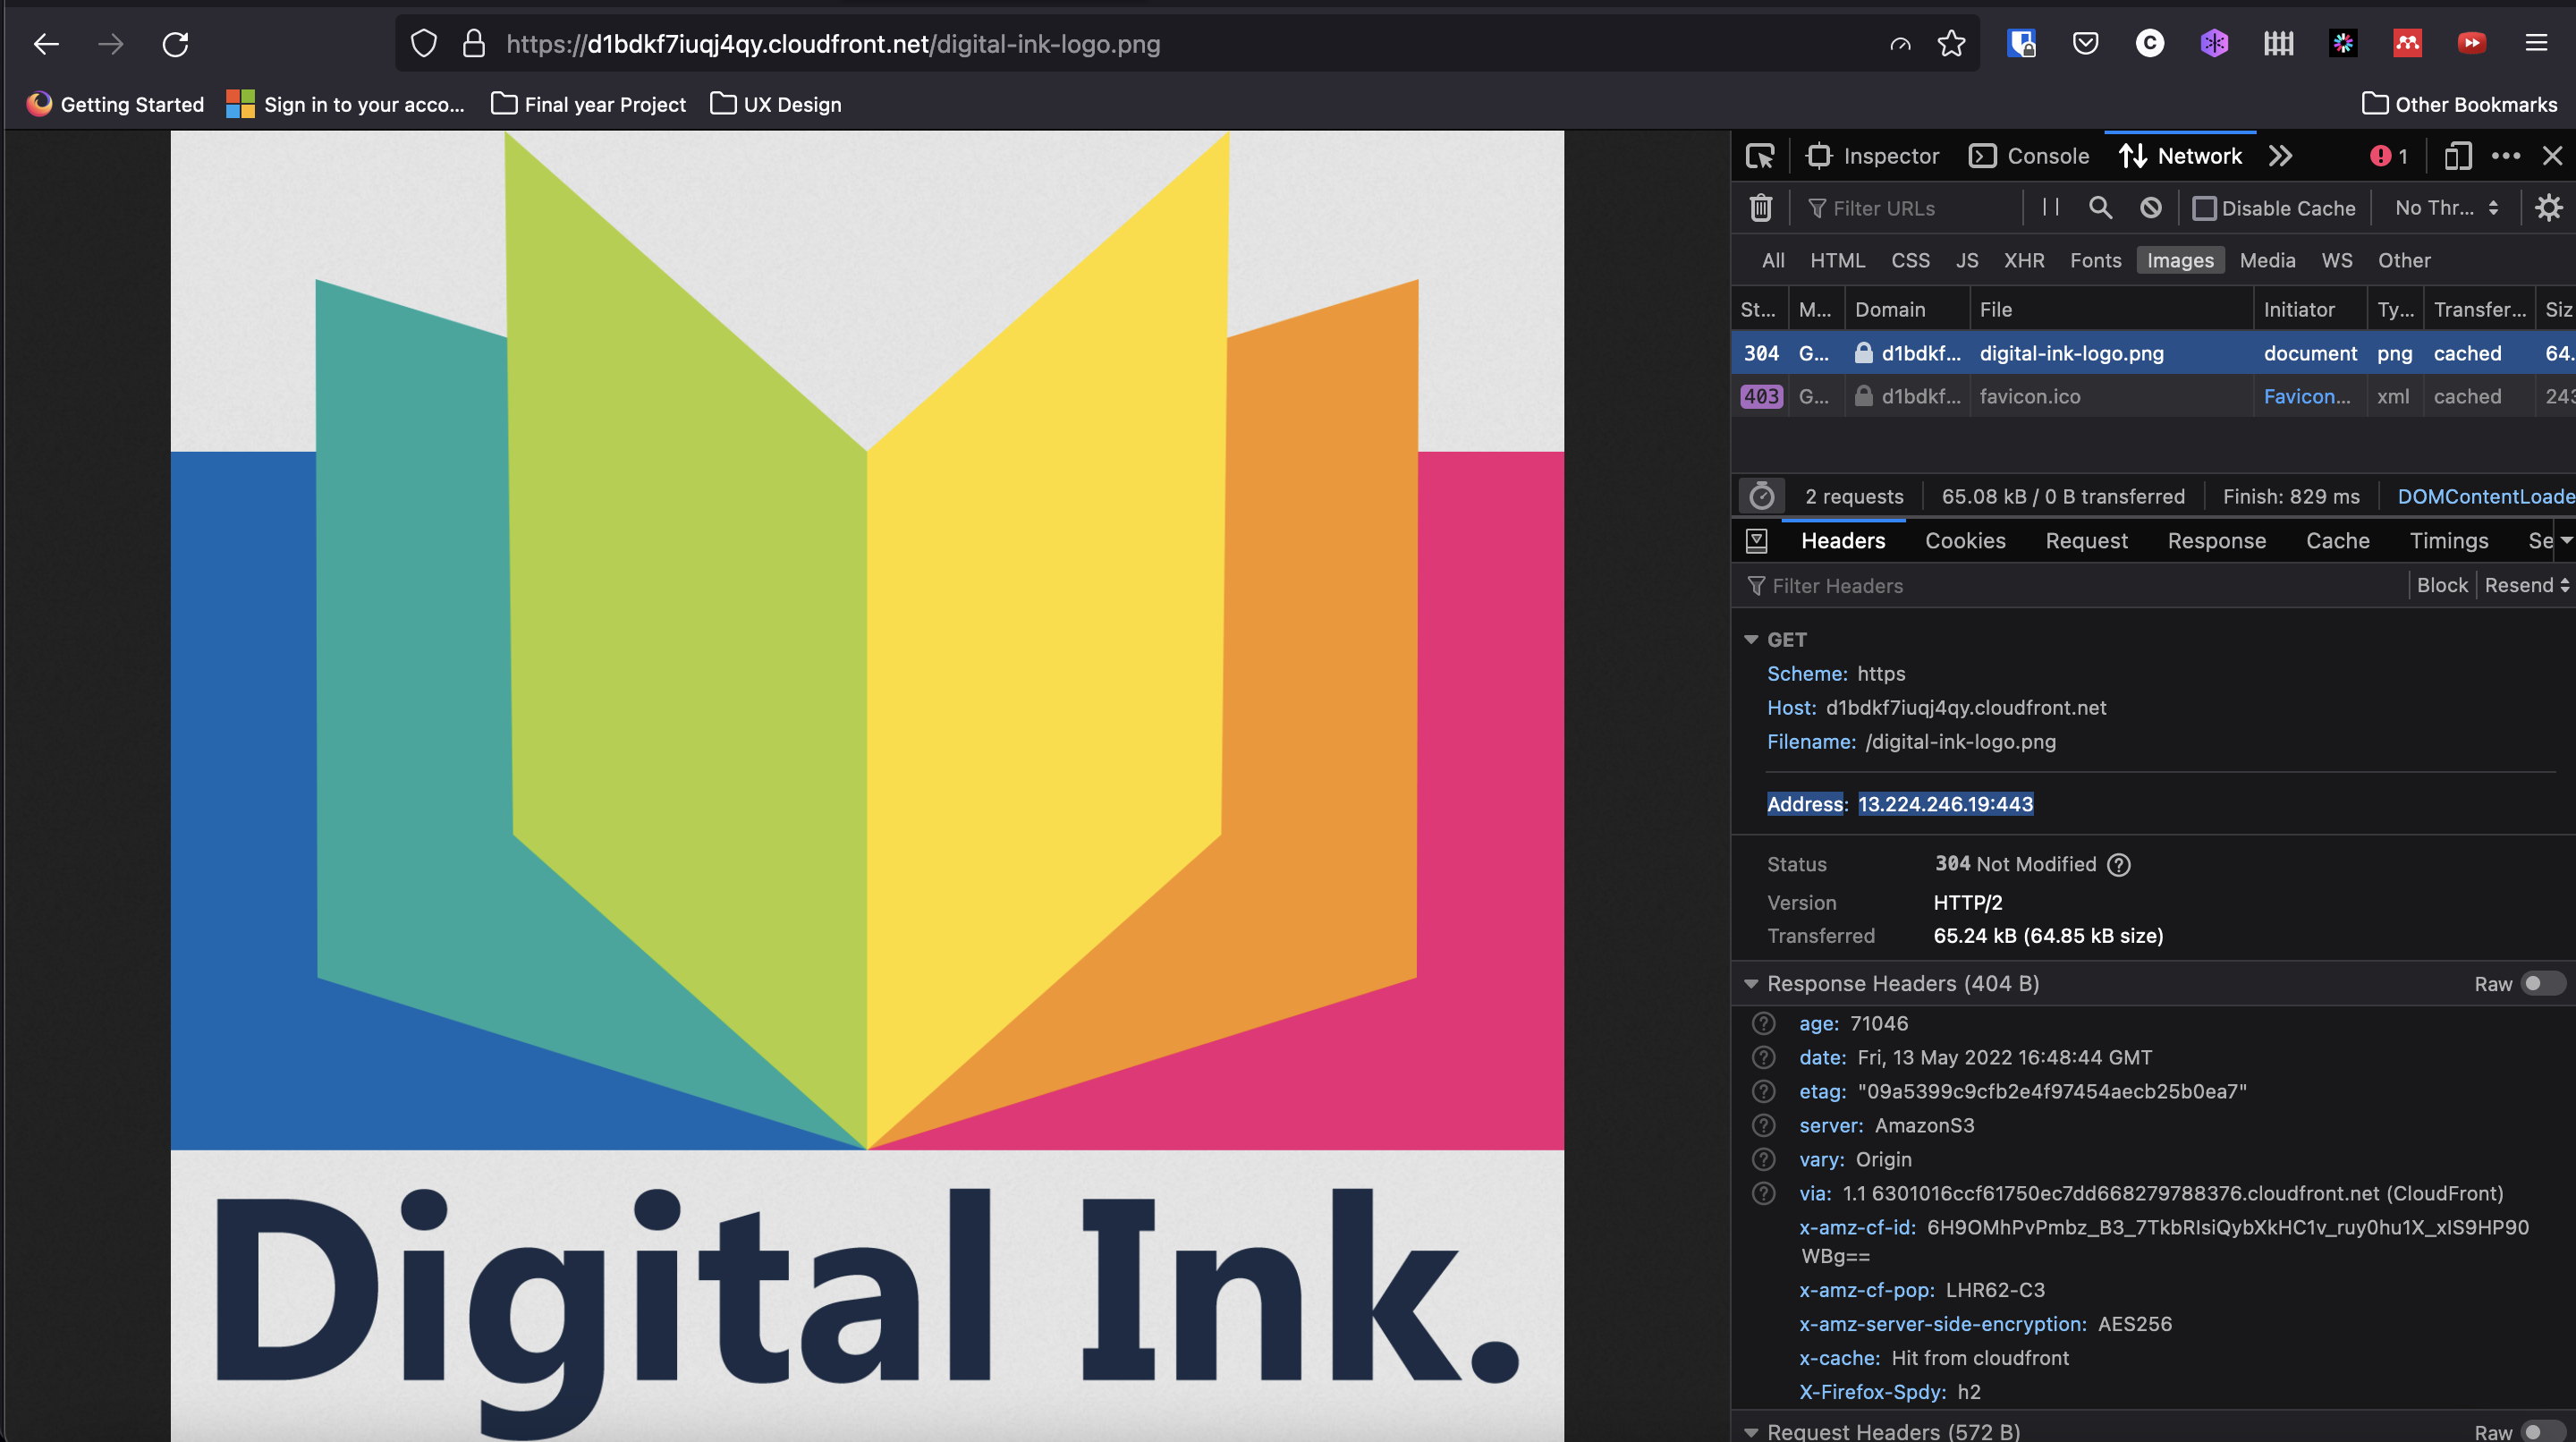
\includegraphics[width=\textwidth]{resources/cloudfront/cloudfront-test-uk}
    \caption{Digital Ink image whilst connected to UK IP.}
    \label{fig:cloudfront-test--uk}
\end{figure}

\begin{figure}[!htbp]
    \centering
    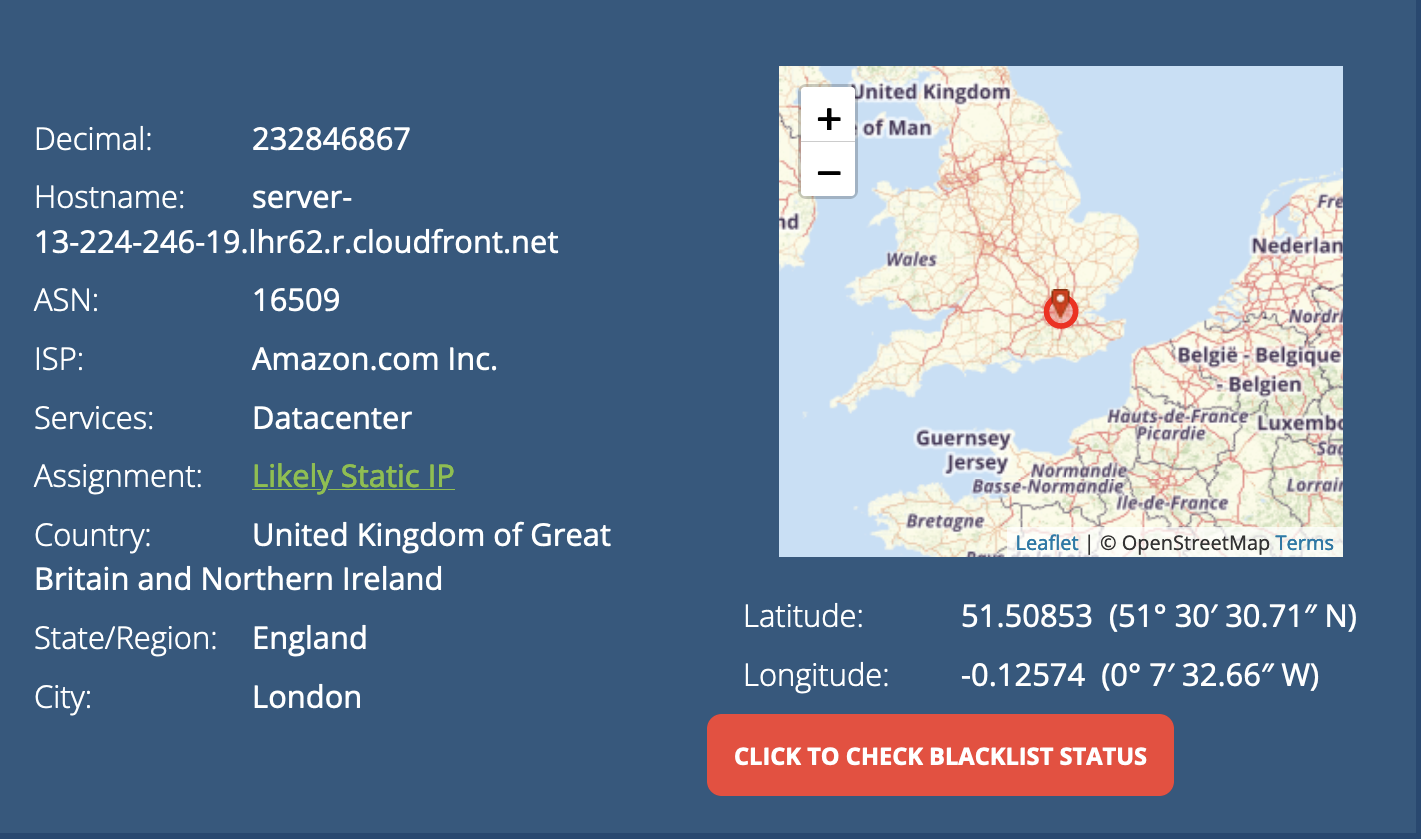
\includegraphics[width=\textwidth]{resources/cloudfront/cloudfront-test-uk-ip}
    \caption{UK IP Location.}
    \label{fig:cloudfront-test-uk-ip}
\end{figure}

\begin{figure}[!htbp]
    \centering
    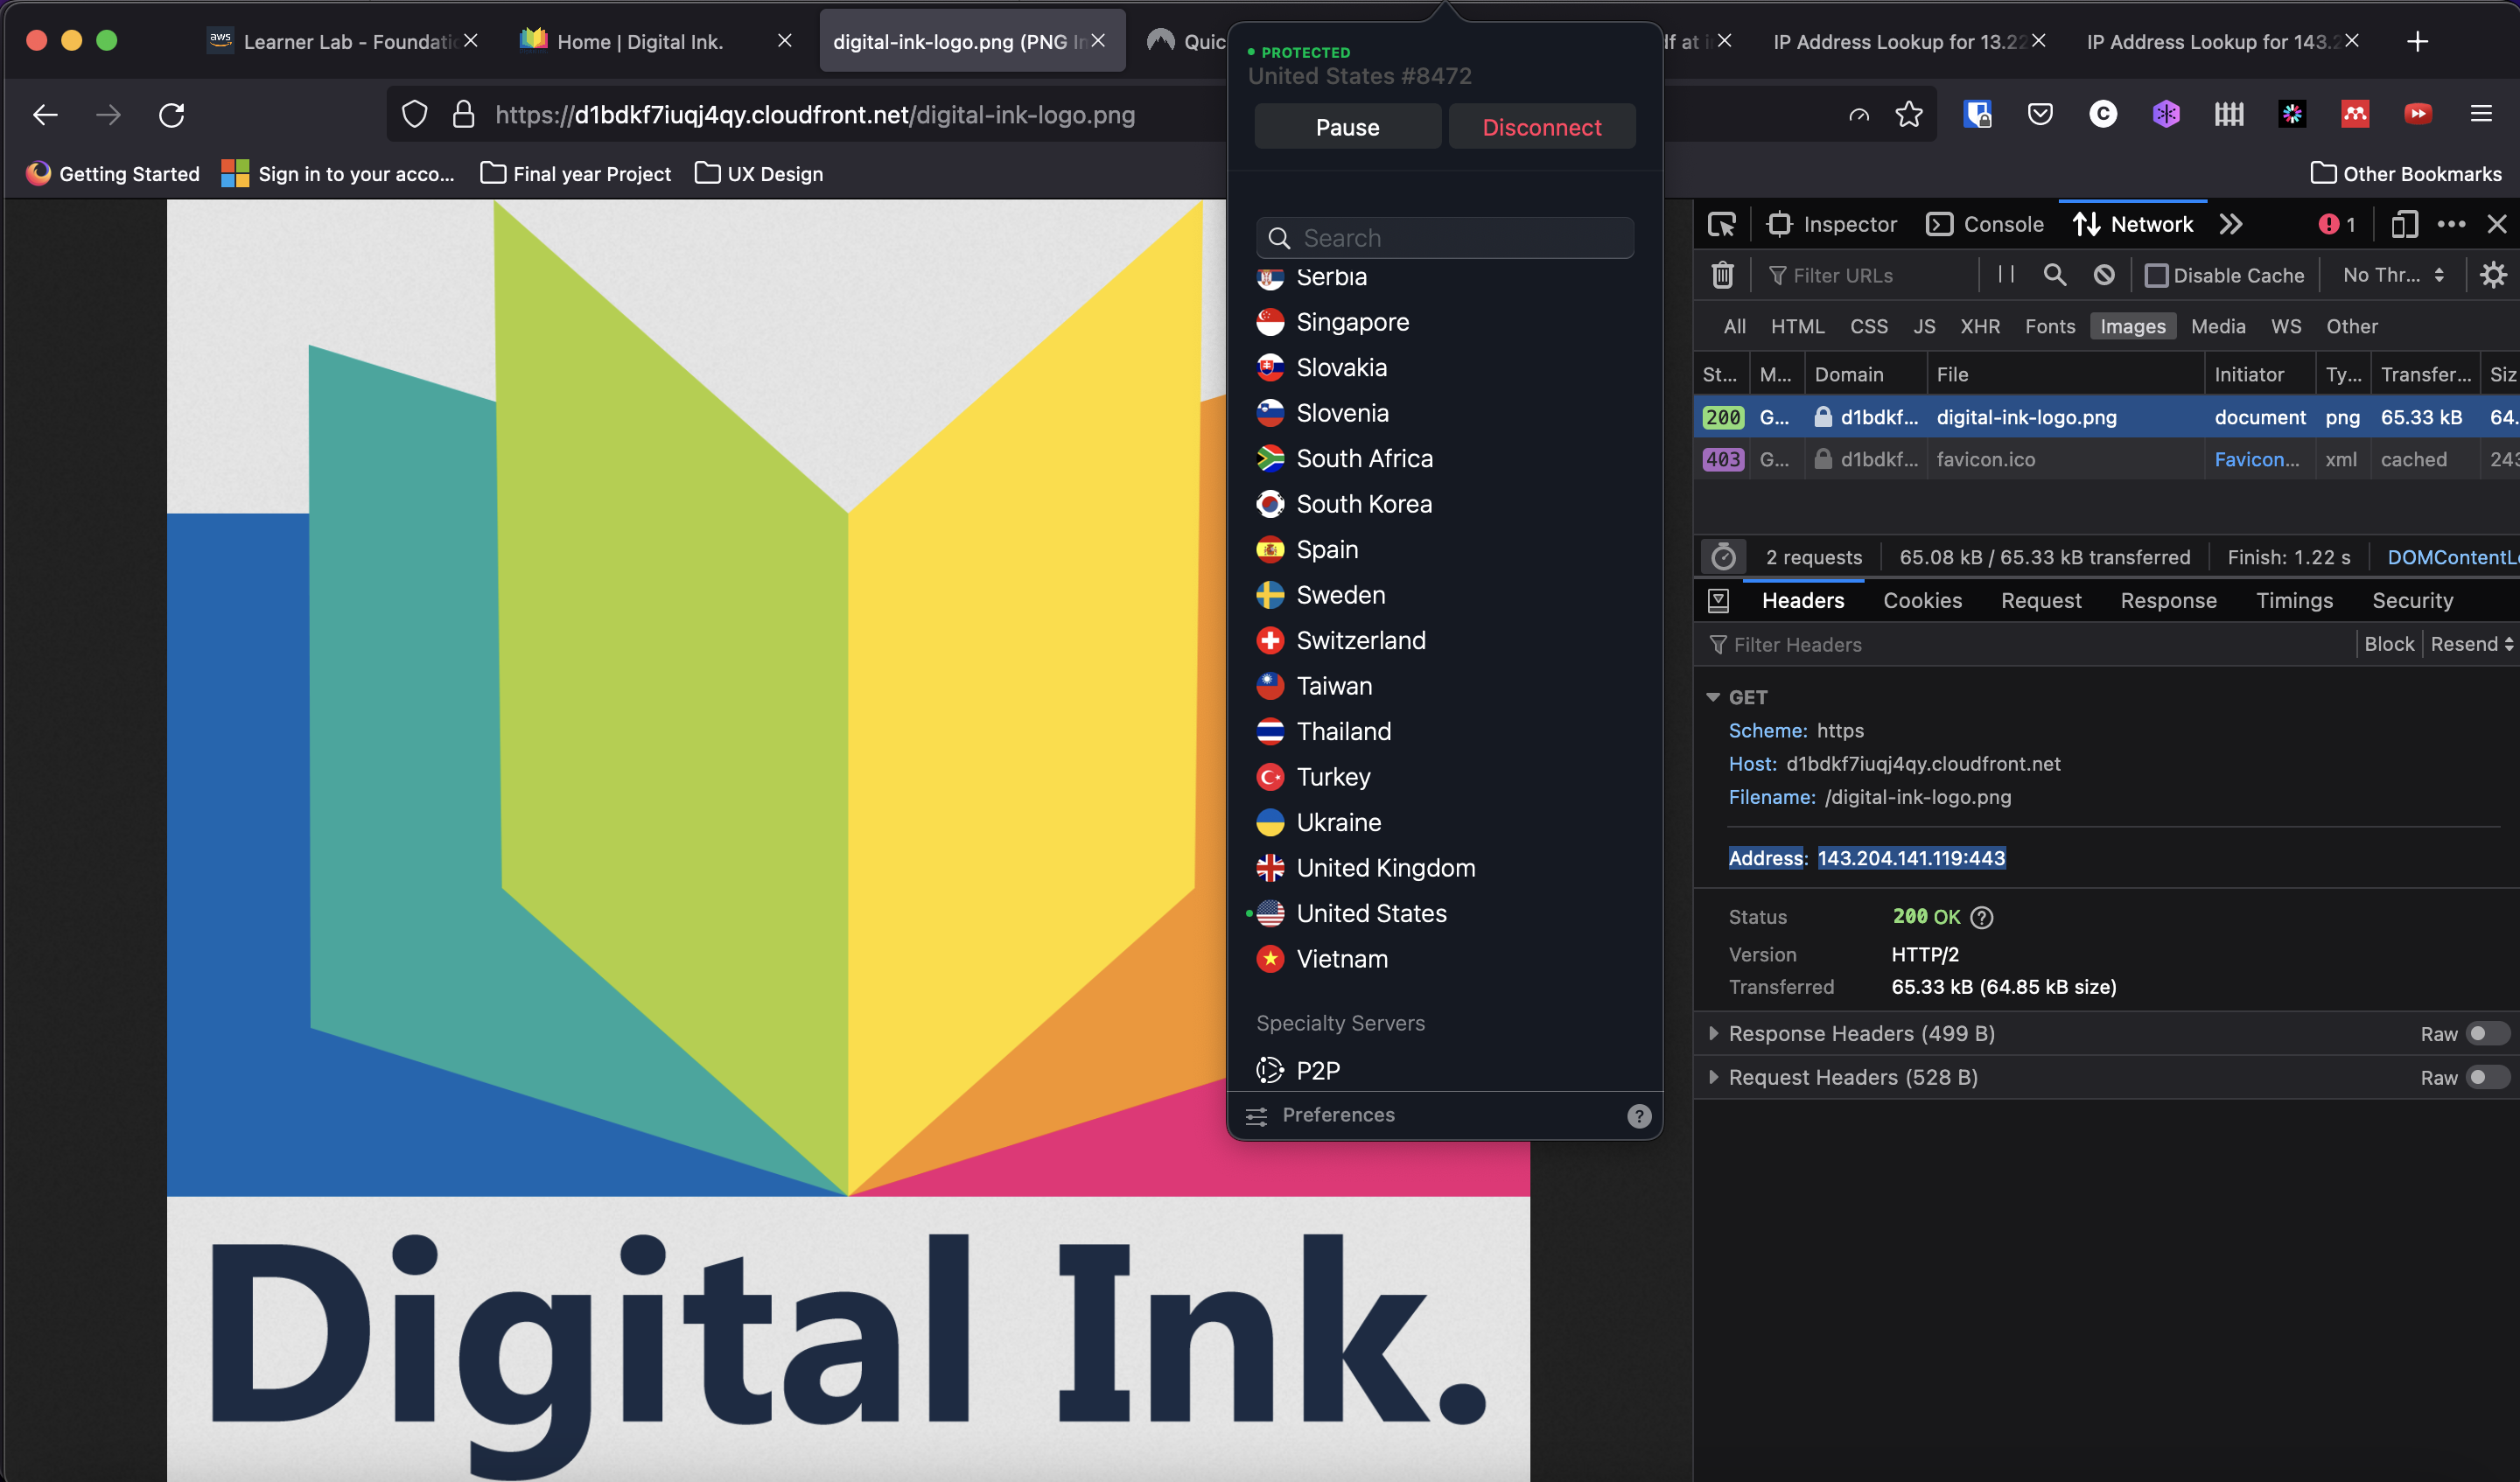
\includegraphics[width=\textwidth]{resources/cloudfront/cloudfront-test-us}
    \caption{Digital Ink image whilst connected to US IP.}
    \label{fig:cloudfront-test-us}
\end{figure}

\begin{figure}[!htbp]
    \centering
    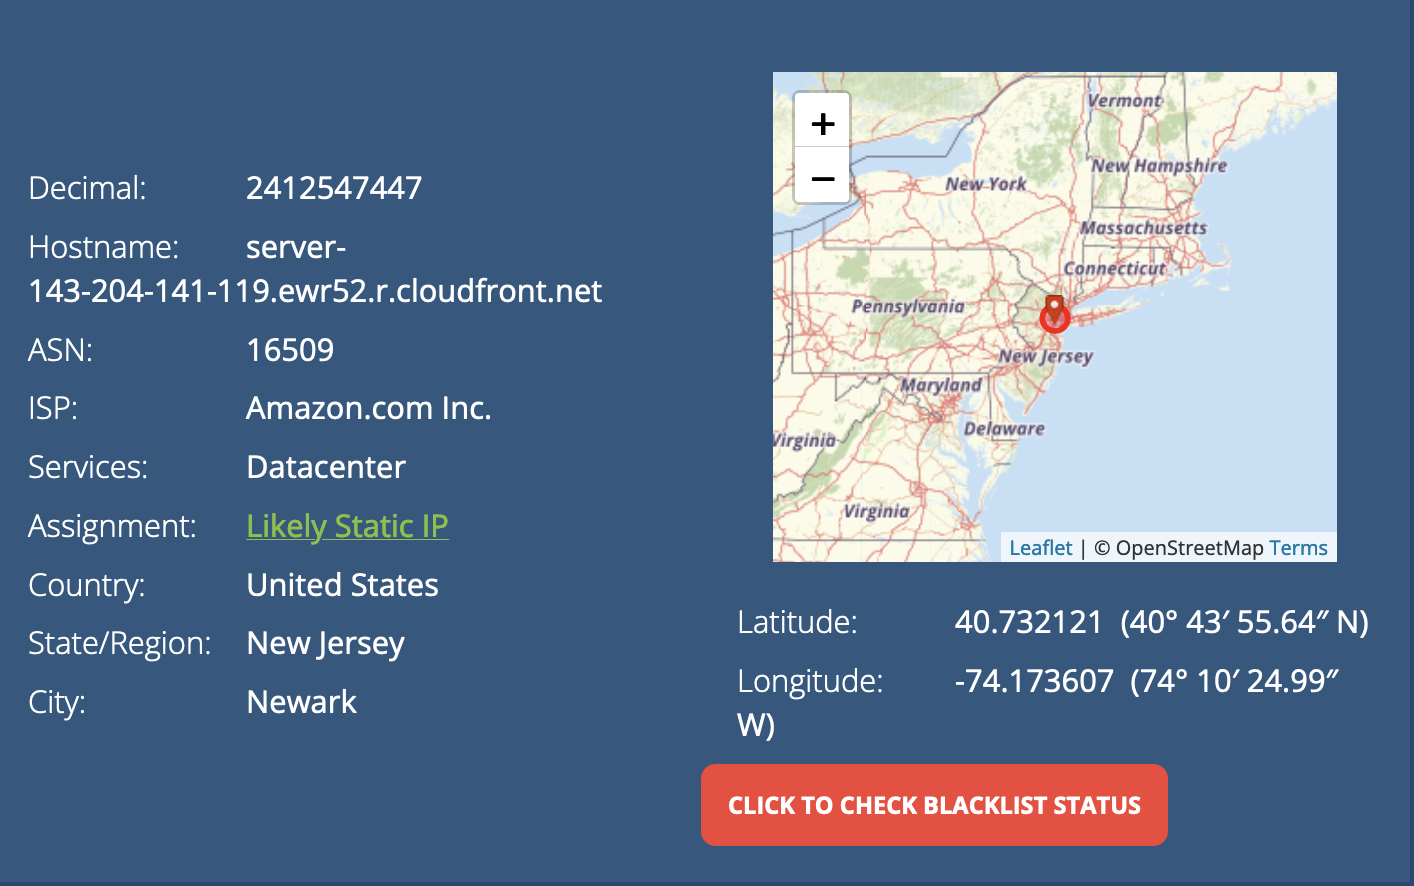
\includegraphics[width=\textwidth]{resources/cloudfront/cloudfront-test-us-ip}
    \caption{US IP Location.}
    \label{fig:cloudfront-test-us-ip}
\end{figure}

\clearpage
\section{Testing RDS}\label{sec:testing-rds}
\begin{figure}[!htbp]
    \centering
    \begin{minted}{cucumber}
Scenario: Creating user information through the web app.
    Given that the user does not have an account on the web app
    When the user creates an account through the web app
    Then their account will be added to the users table on the RDS instance
    \end{minted}
    \label{fig:create-user-data}
\end{figure}

\begin{figure}[!htbp]
    \centering
    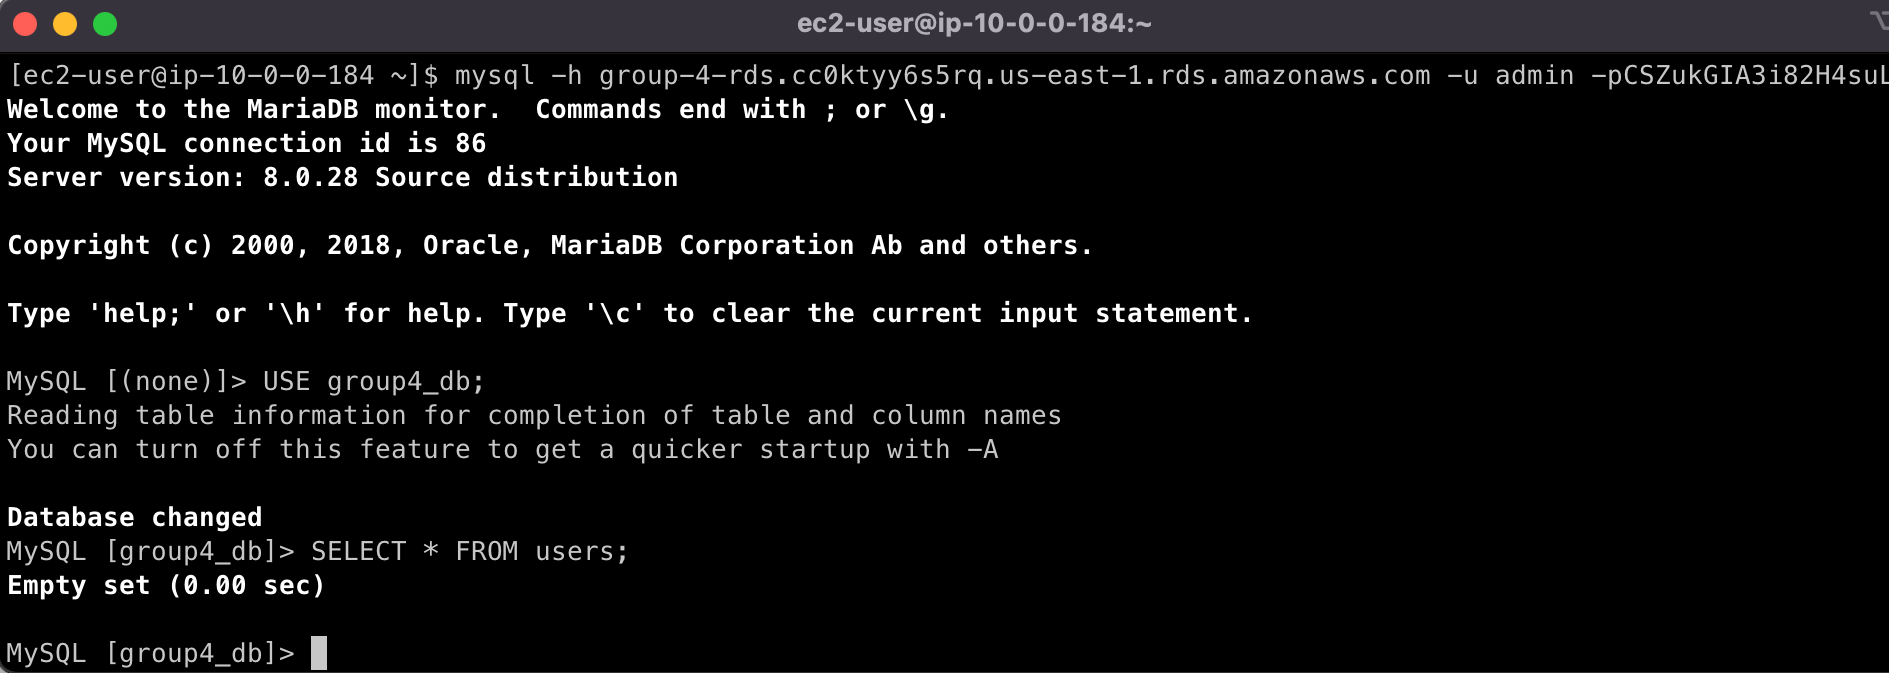
\includegraphics[width=\textwidth]{resources/rds/rds-testing-empty}
    \caption{Empty users table before test.}
    \label{fig:rds-testing-empty}
\end{figure}

\begin{figure}[!htbp]
    \centering
    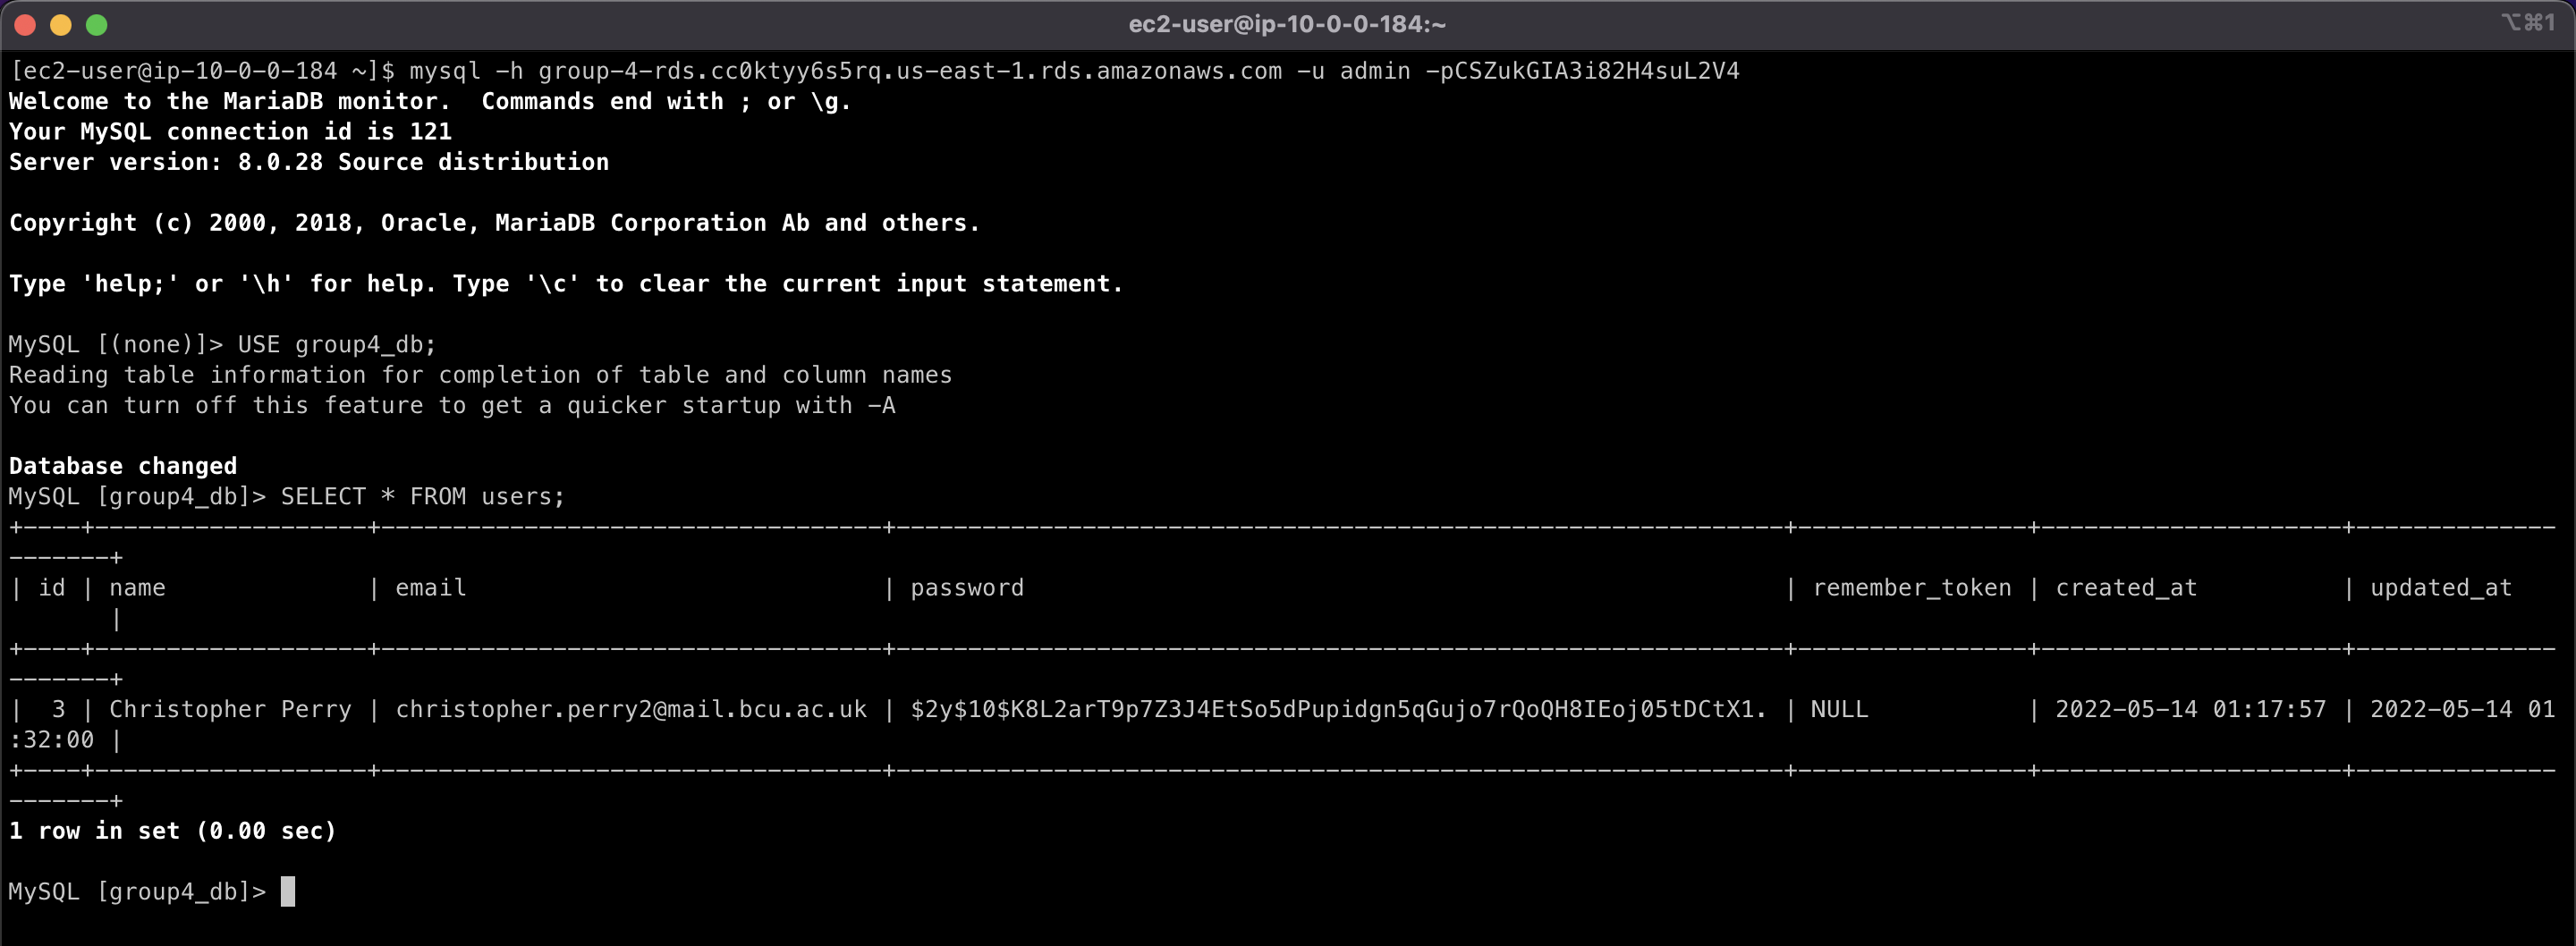
\includegraphics[width=\textwidth]{resources/rds/rds-testing-user-added}
    \caption{Users table now populated after test.}
    \label{fig:rds-testing-user-added}
\end{figure}

\clearpage
\begin{figure}[!htbp]
    \centering
    \begin{minted}{cucumber}
Scenario: Creating story information through the web app.
    Given the user has a digital ink account
    When they create a story on the website
    Then their story will be added to the stories table on the RDS instance
    \end{minted}
    \label{fig:create-story-data}
\end{figure}

\begin{figure}[!htbp]
    \centering
    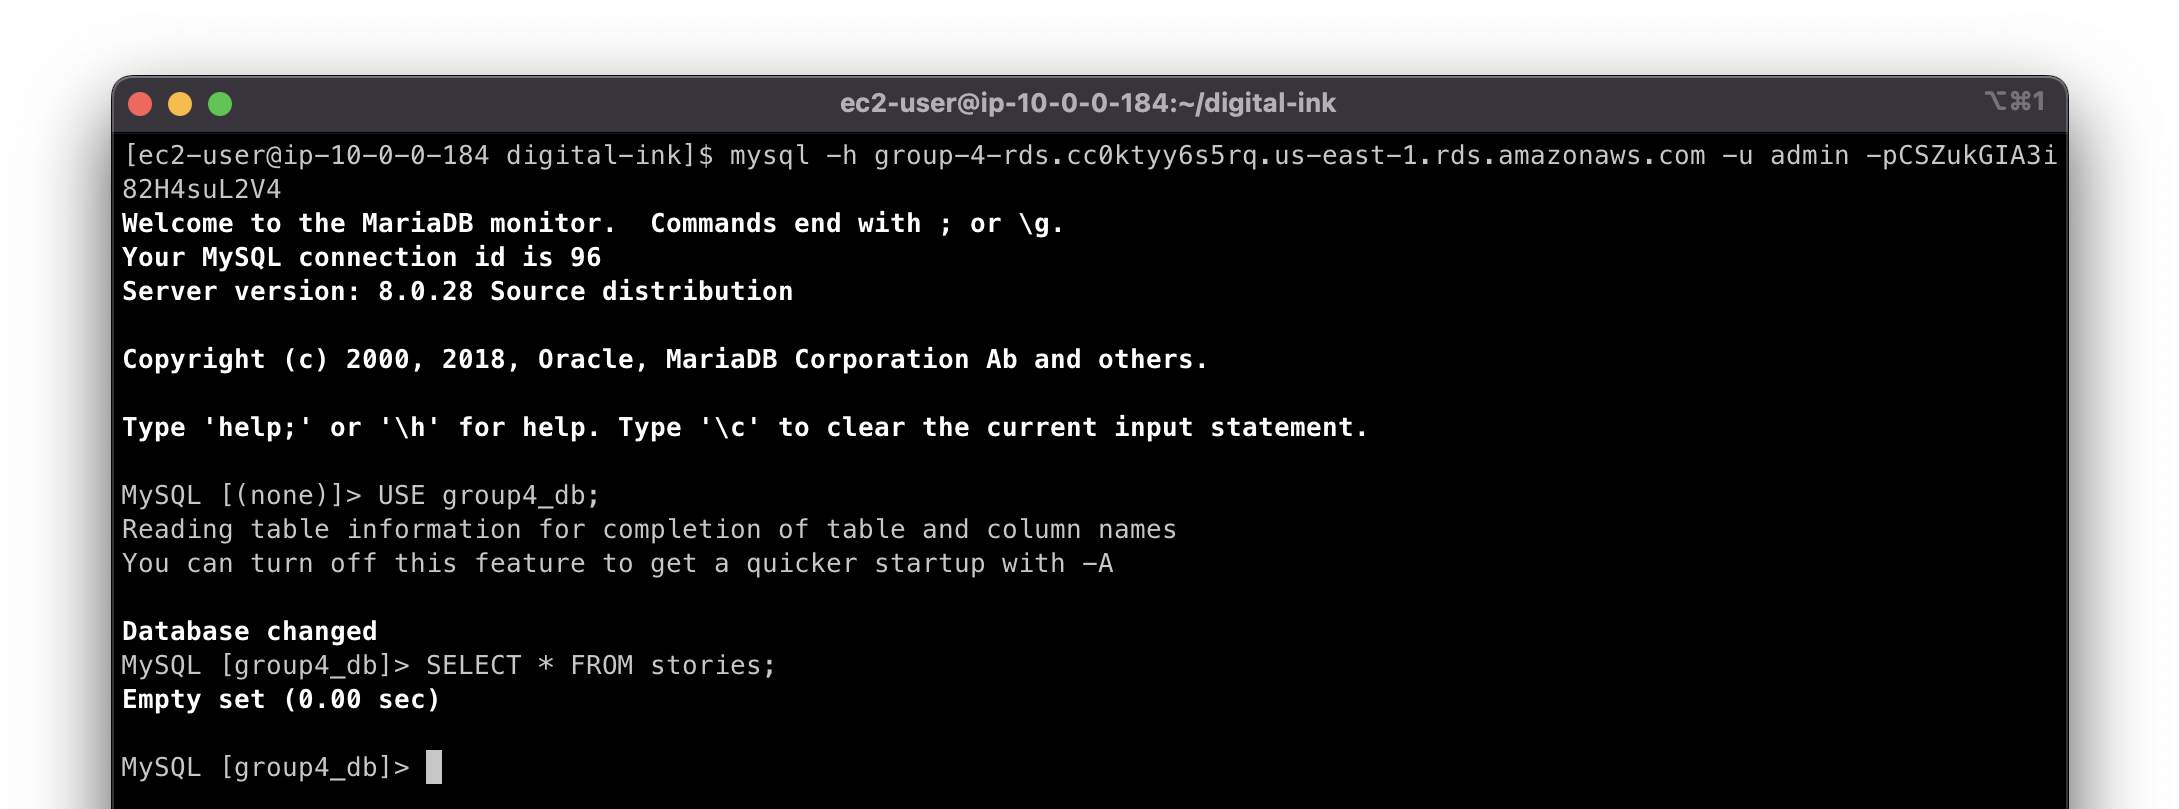
\includegraphics[width=\textwidth]{resources/rds/rds-testing-stories-before}
    \caption{Empty stories table before test.}
    \label{fig:rds-testing-stories-empty}
\end{figure}

\begin{figure}[!htbp]
    \centering
    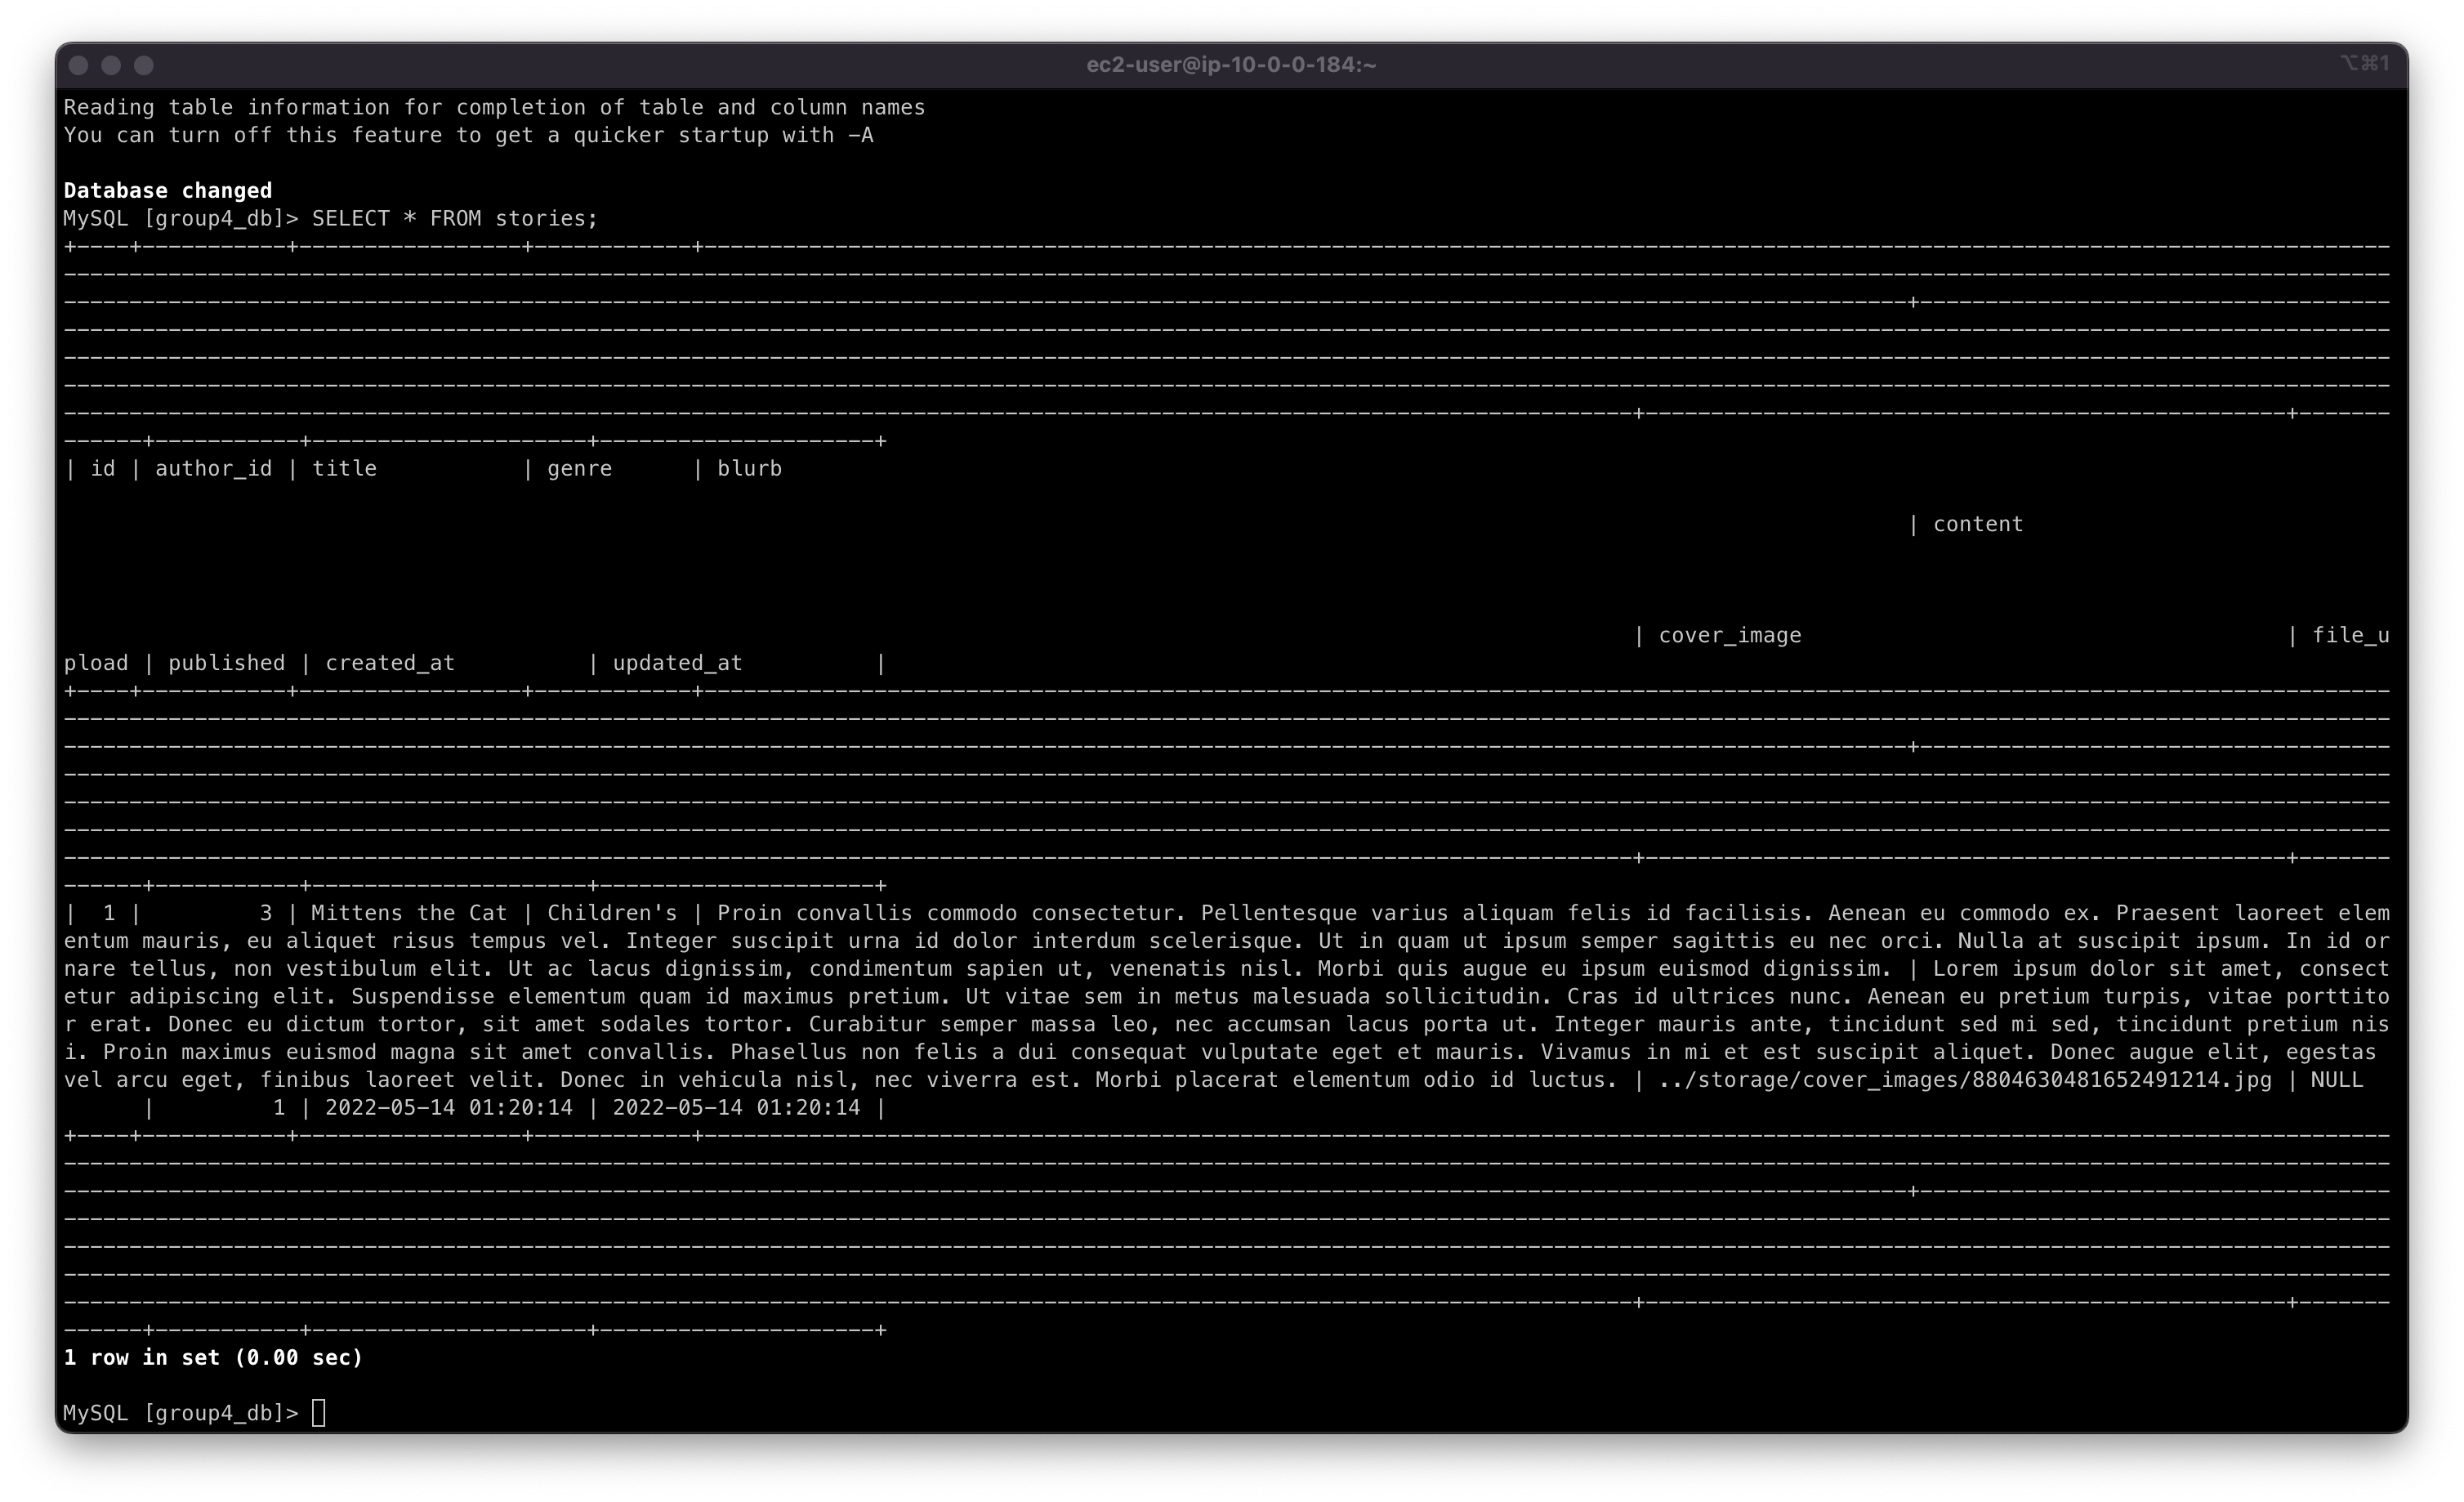
\includegraphics[width=\textwidth]{resources/rds/rds-testing-stories-after}
    \caption{Stories table now populated after test.}
    \label{fig:rds-testing-story-added}
\end{figure}

\clearpage
\begin{figure}[!htbp]
    \centering
    \begin{minted}{cucumber}
Scenario: Updating user information in the database through the web app.
    Given the user has an account in the web app
    When they change their name and email
    Then the information will be updated in the users table in the RDS instance
    \end{minted}
    \label{fig:update-user-data}
\end{figure}

\begin{figure}[!htbp]
    \centering
    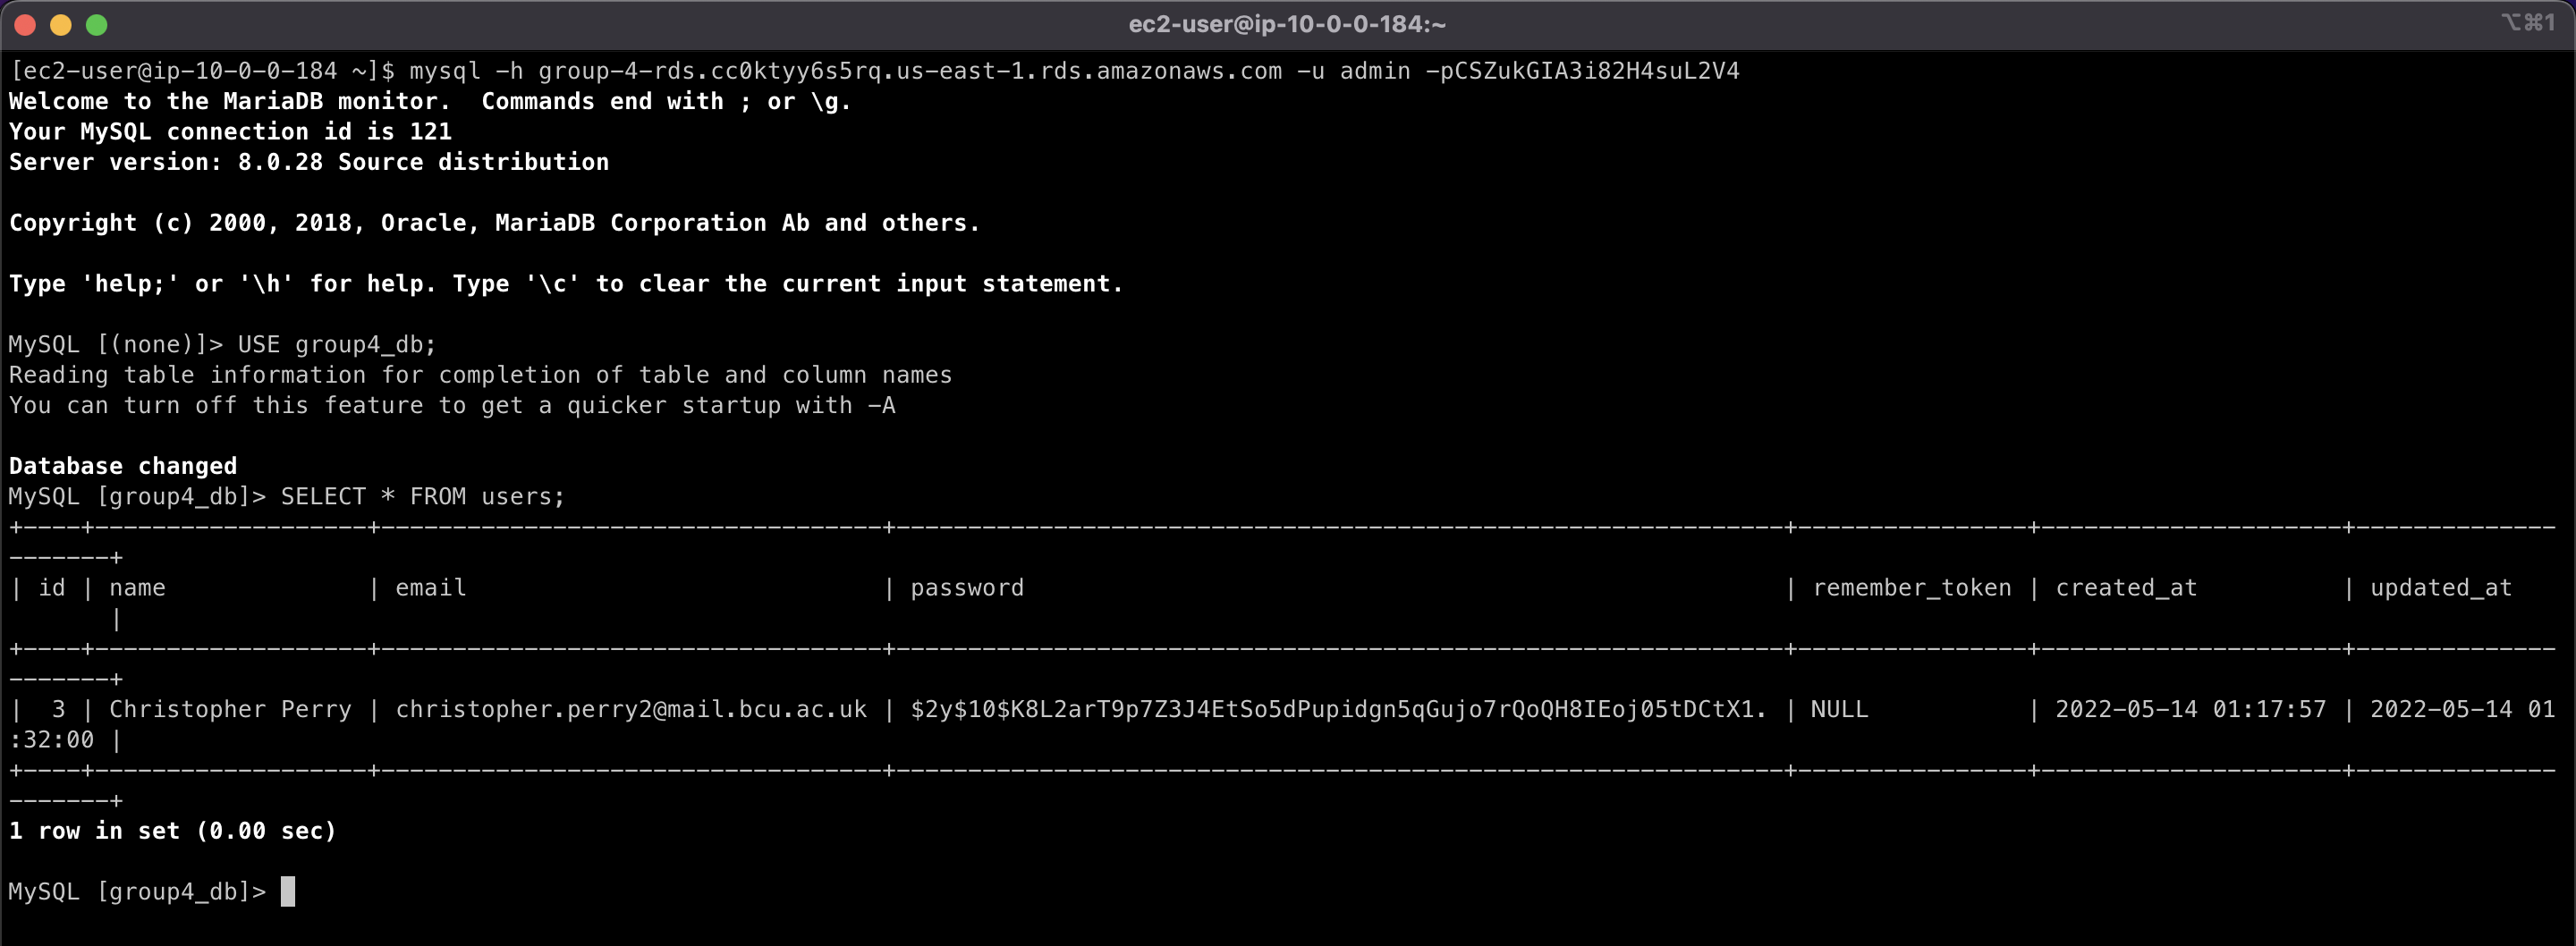
\includegraphics[width=\textwidth]{resources/rds/rds-testing-user-added}
    \caption{User before update.}
    \label{fig:rds-testing-user-before-update}
\end{figure}

\begin{figure}[!htbp]
    \centering
    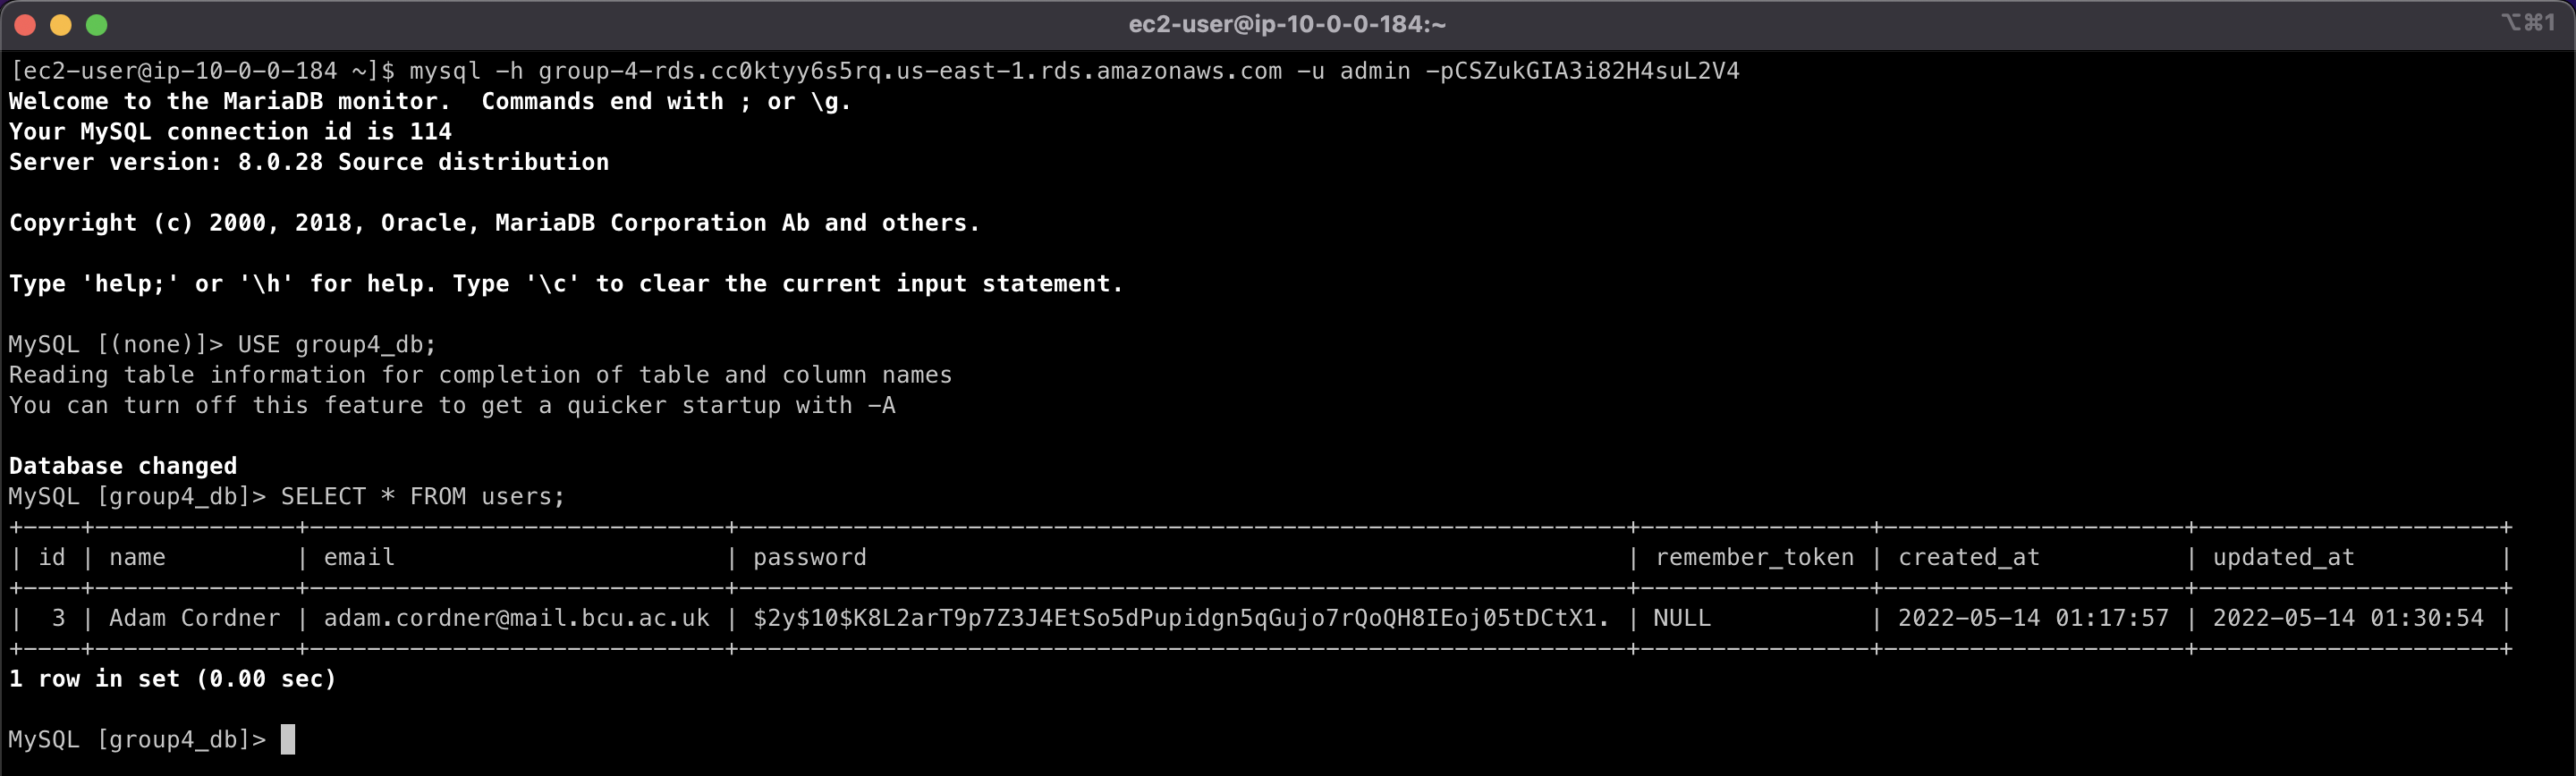
\includegraphics[width=\textwidth]{resources/rds/rds-testing-update-after}
    \caption{User after update. Notice that the hashed password remains the same.}
    \label{fig:rds-testing-user-after-update}
\end{figure}

\clearpage
\begin{figure}[!htbp]
    \centering
    \begin{minted}{cucumber}
Scenario: Deleting story information in the database through the web app.
    Given the user has an account and a story on the web app
    When they delete a story associated with their account
    Then the story will be removed from the stories table in the RDS instance
    \end{minted}
    \label{fig:delete-story-data}
\end{figure}

\begin{figure}[!htbp]
    \centering
    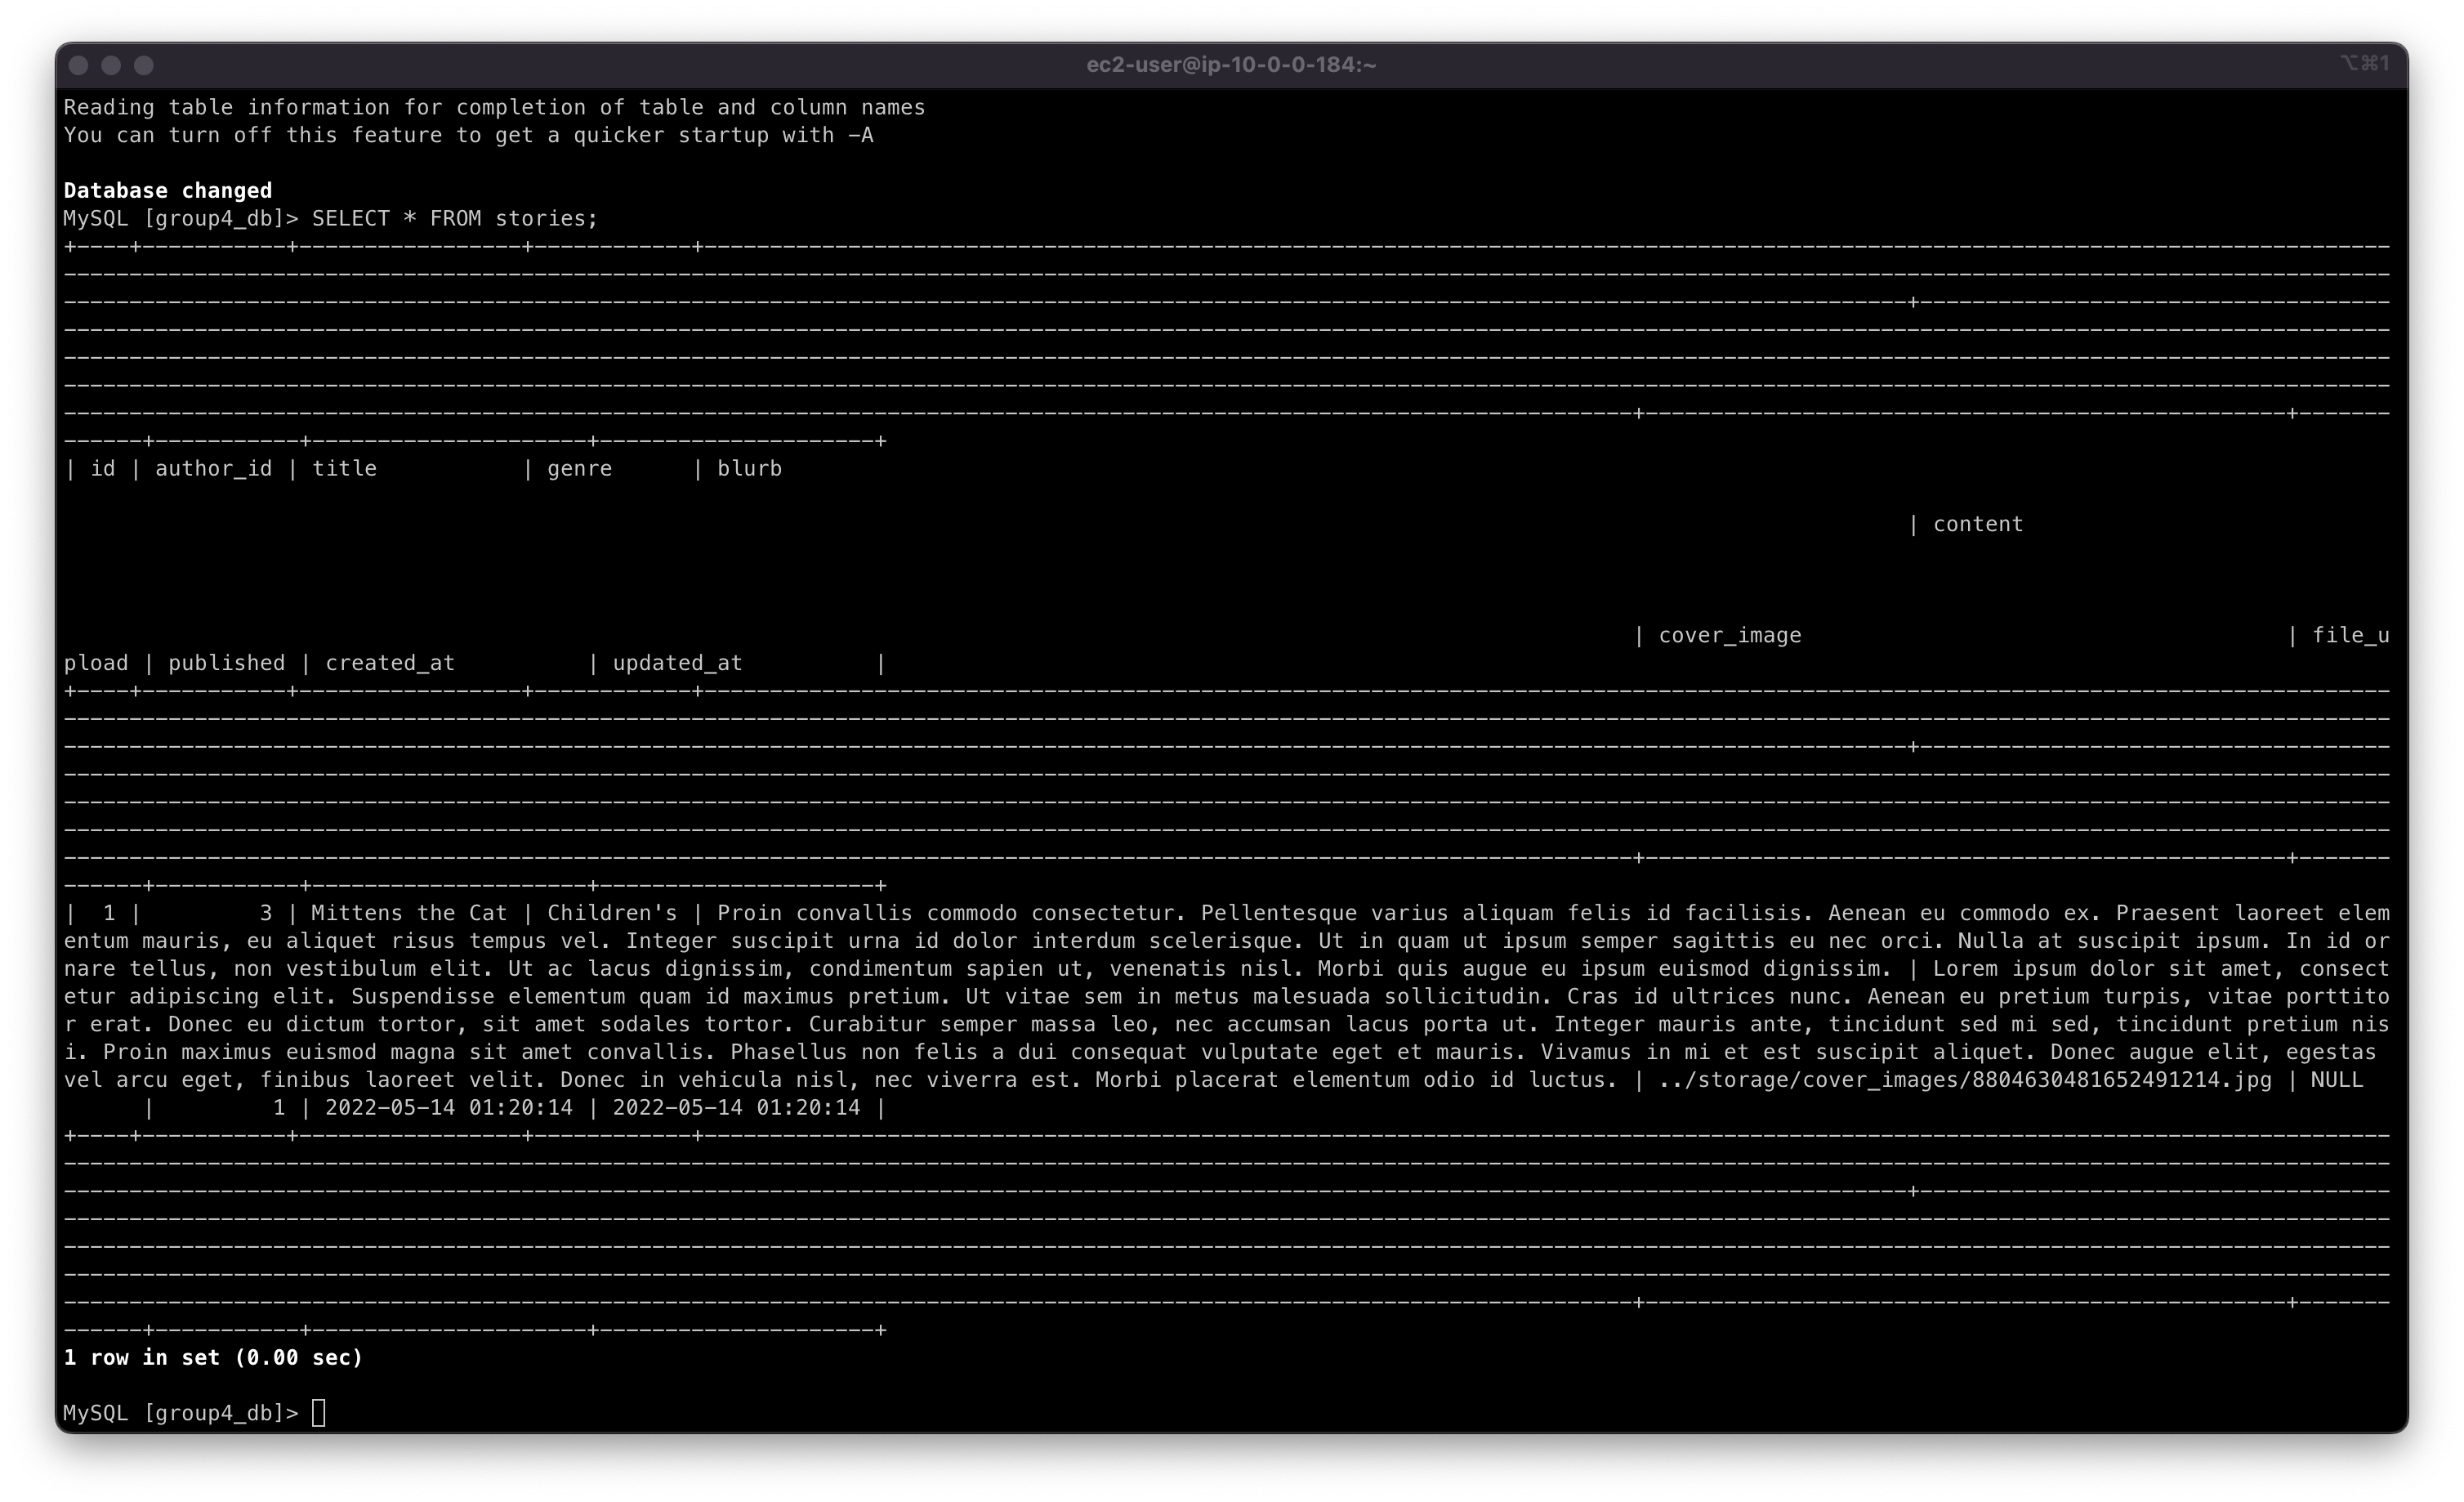
\includegraphics[width=\textwidth]{resources/rds/rds-testing-stories-after}
    \caption{Stories table before deletion.}
    \label{fig:rds-testing-before-story-deletion}
\end{figure}

\begin{figure}[!htbp]
    \centering
    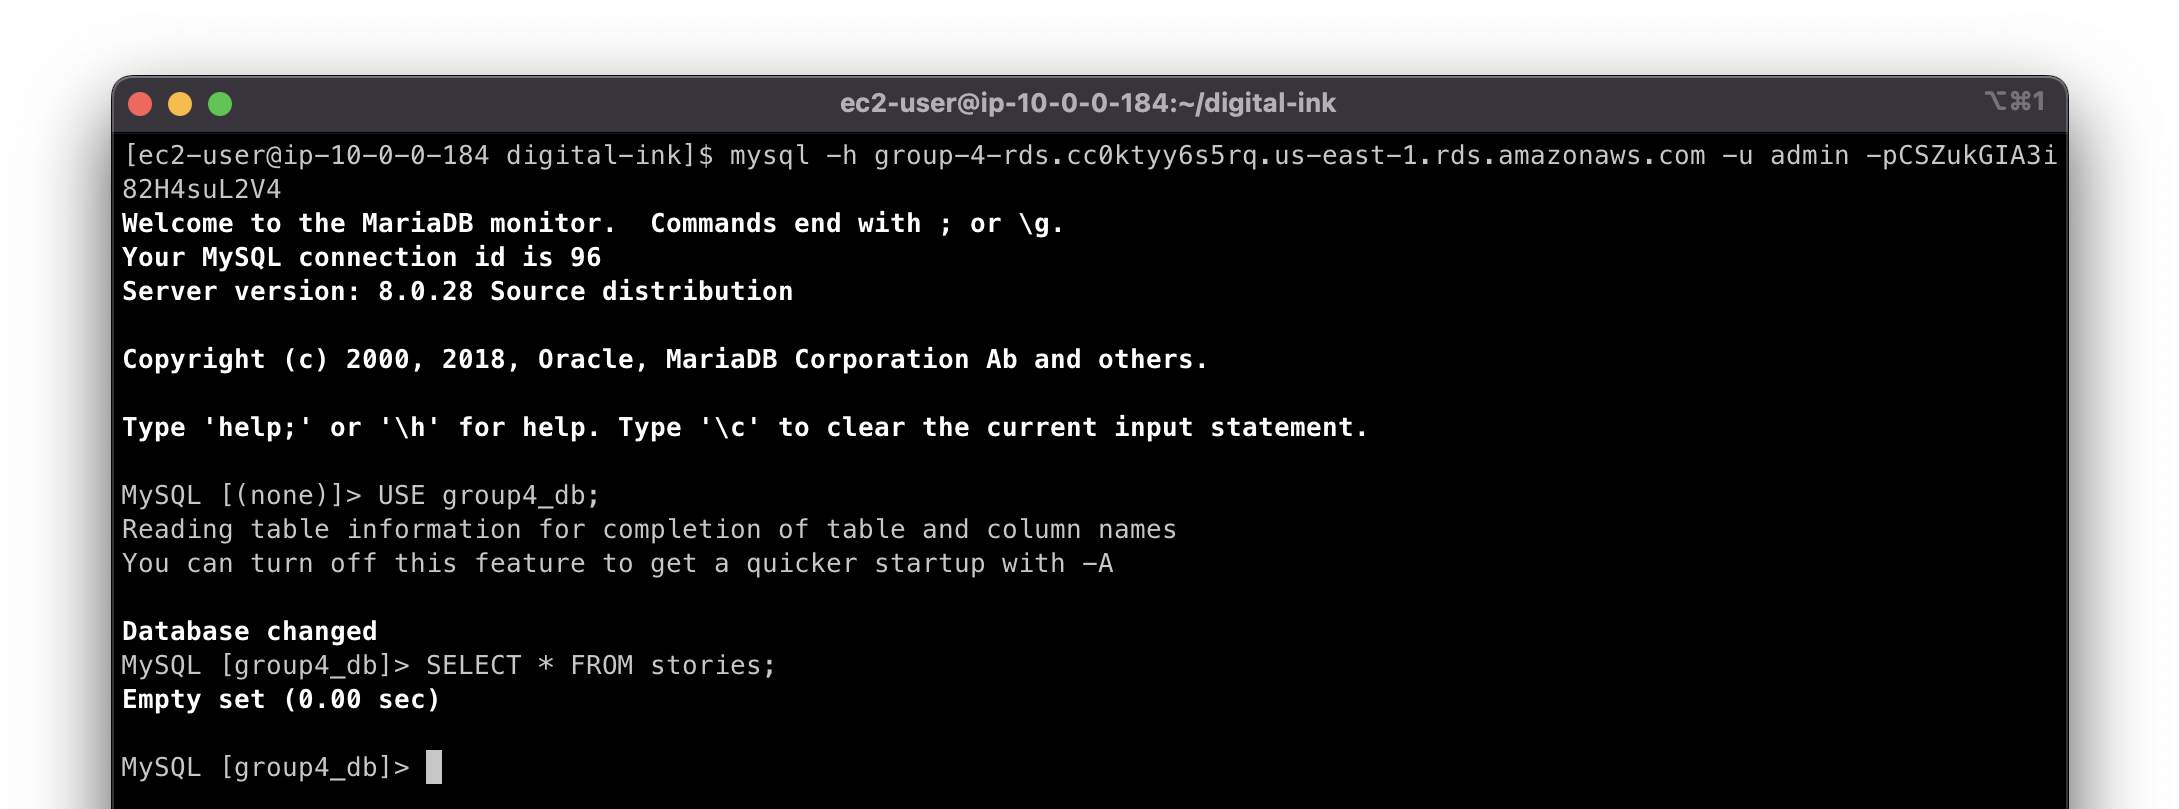
\includegraphics[width=\textwidth]{resources/rds/rds-testing-stories-before}
    \caption{Stories table after deletion.}
    \label{fig:rds-testing-after-story-deletion}
\end{figure}

\clearpage
\section{Testing CloudWatch}\label{sec:testing-cloudwatch}
For the purposes of these tests, alarms were purposefully activated.

\begin{figure}[!htbp]
    \centering
    \begin{minted}{cucumber}
Scenario: Testing that NetworkAlarm activates
    Given that the NetworkAlarm is active
    When the EC2 instance outputs more than 500 packets of data
    in 1 minute
    Then the alarm should activate.
    \end{minted}
    \label{fig:cloudwatch-network-alarm-test}
\end{figure}

\begin{figure}[!htbp]
    \centering
    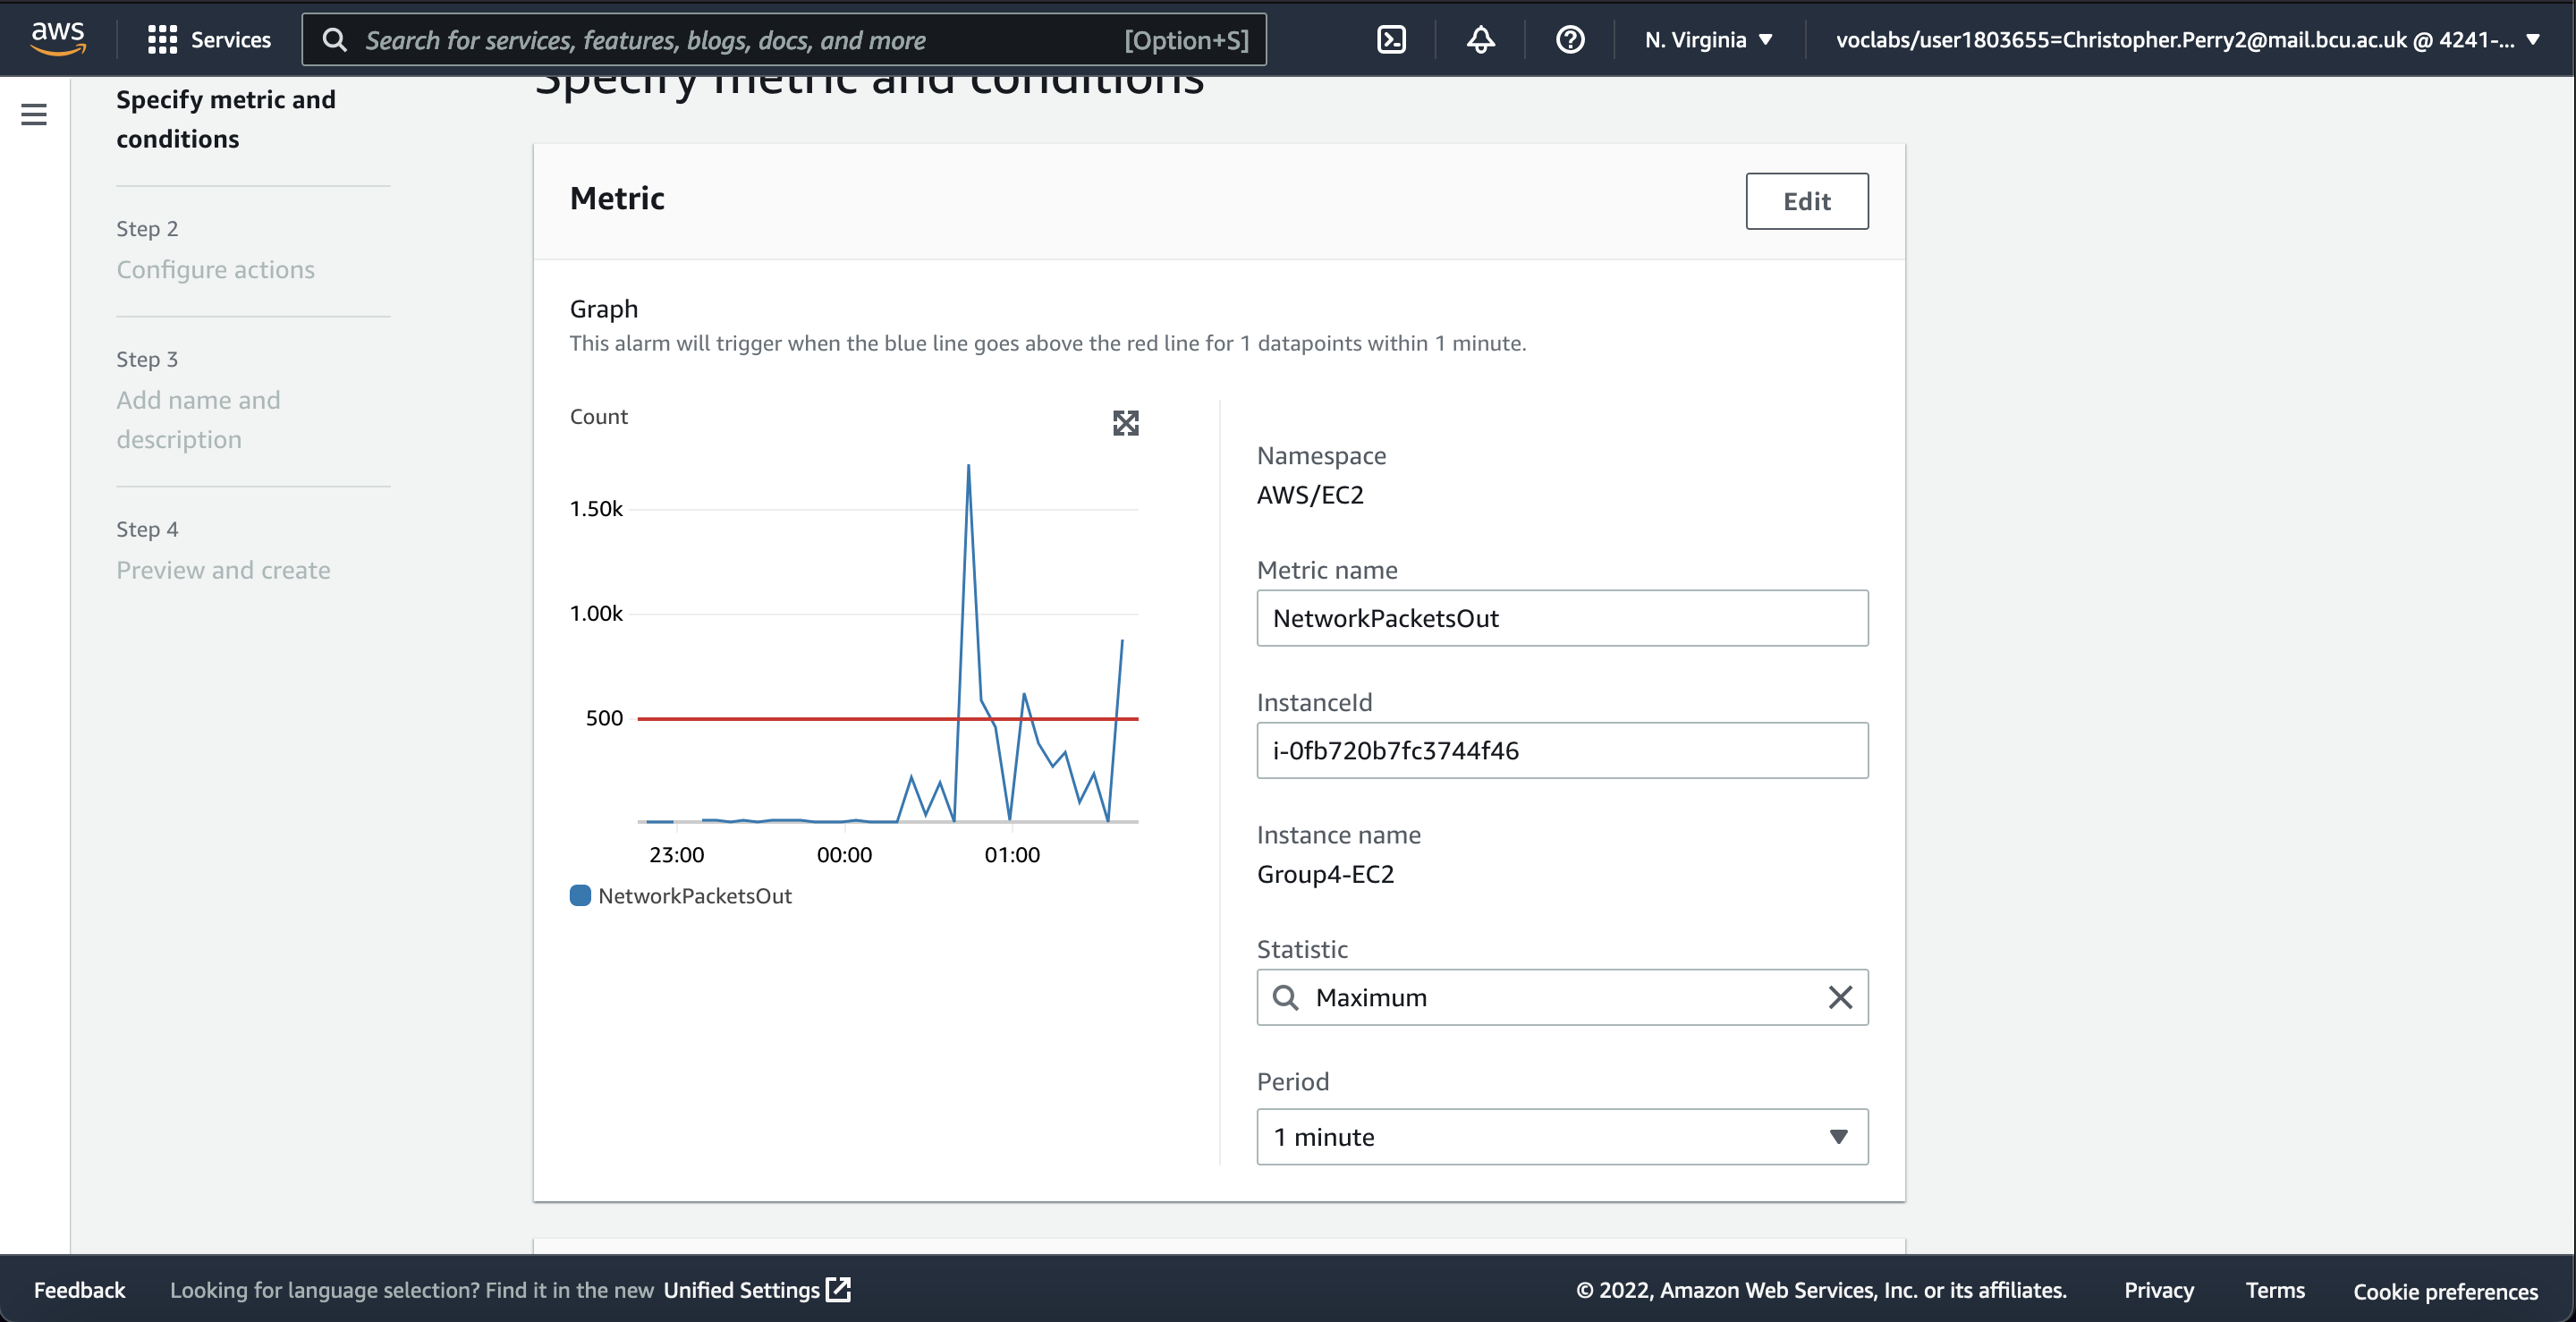
\includegraphics[width=\textwidth]{resources/cloudwatch/cloudwatch-network-alarm-setup}
    \caption{CloudWatch NetworkAlarm setup.}
    \label{fig:cloudwatch-network-alarm-setup}
\end{figure}

\begin{figure}[!htbp]
    \centering
    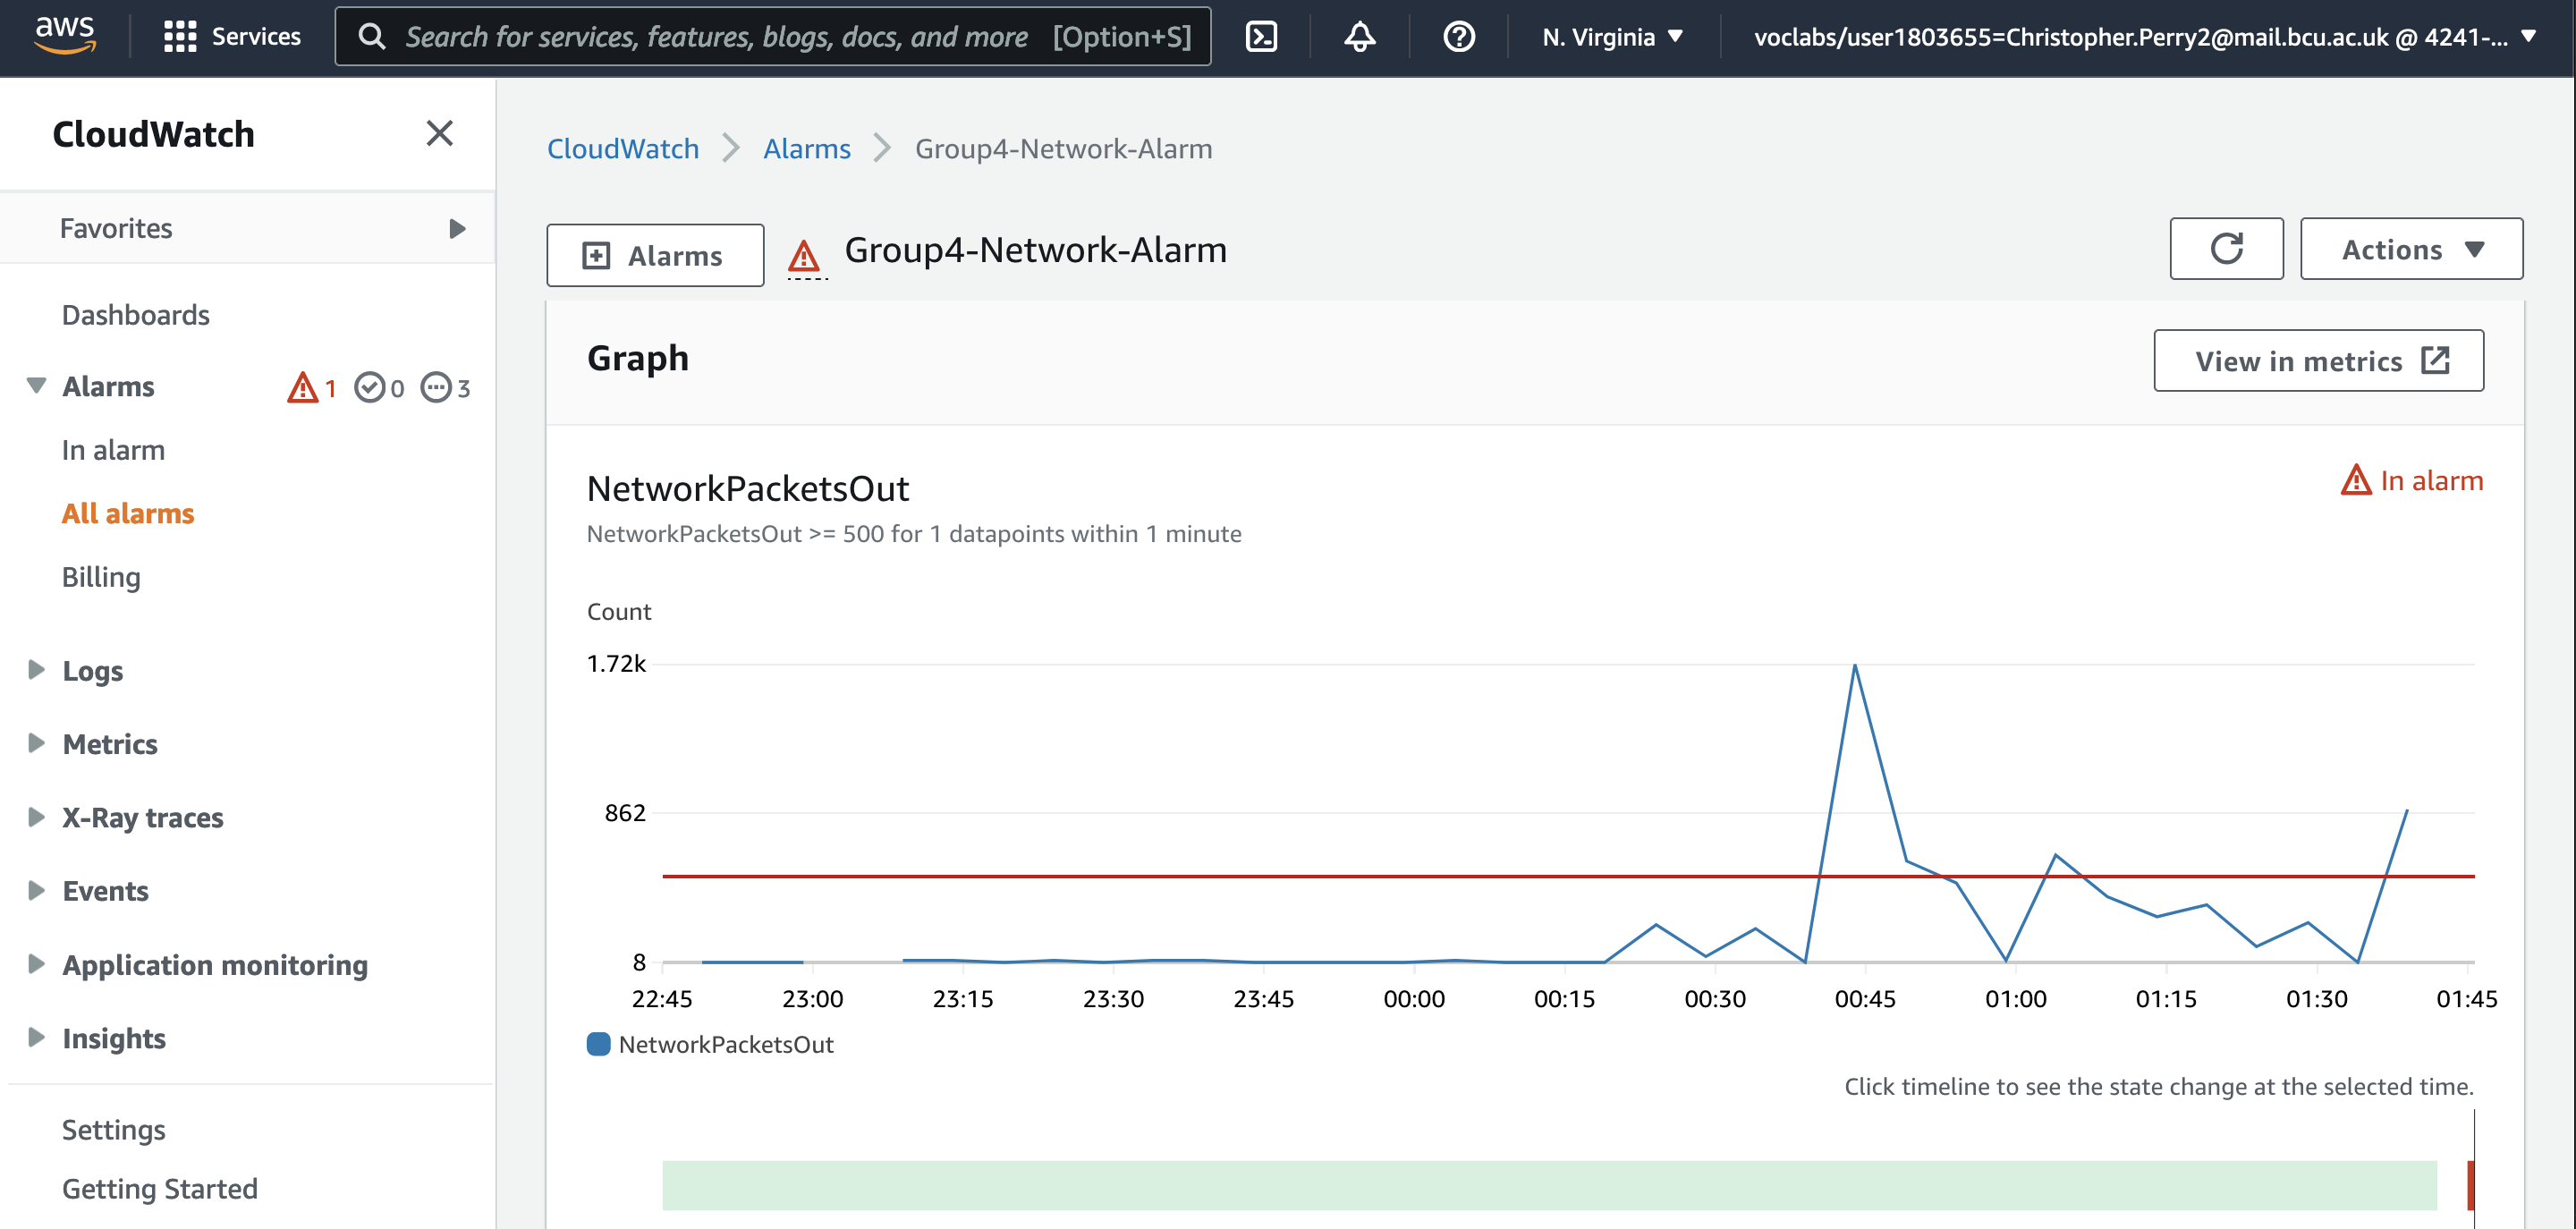
\includegraphics[width=\textwidth]{resources/cloudwatch/cloudwatch-network-alarm-active}
    \caption{CloudWatch NetworkAlarm activated.}
    \label{fig:cloudwatch-network-alarm-active}
\end{figure}

\clearpage

\section{Testing CloudTrail}\label{sec:testing-cloudtrail}
\begin{figure}[!htbp]
    \centering
    \begin{minted}{cucumber}
Scenario: Testing CloudTrail logs RDS activity.
    Given that the Group4-CloudTrail service is active
    When data is added to the RDS database
    Then this information is logged through CloudTrail
    \end{minted}
    \label{fig:cloudtrail-test}
\end{figure}

\begin{figure}[!htbp]
    \centering
    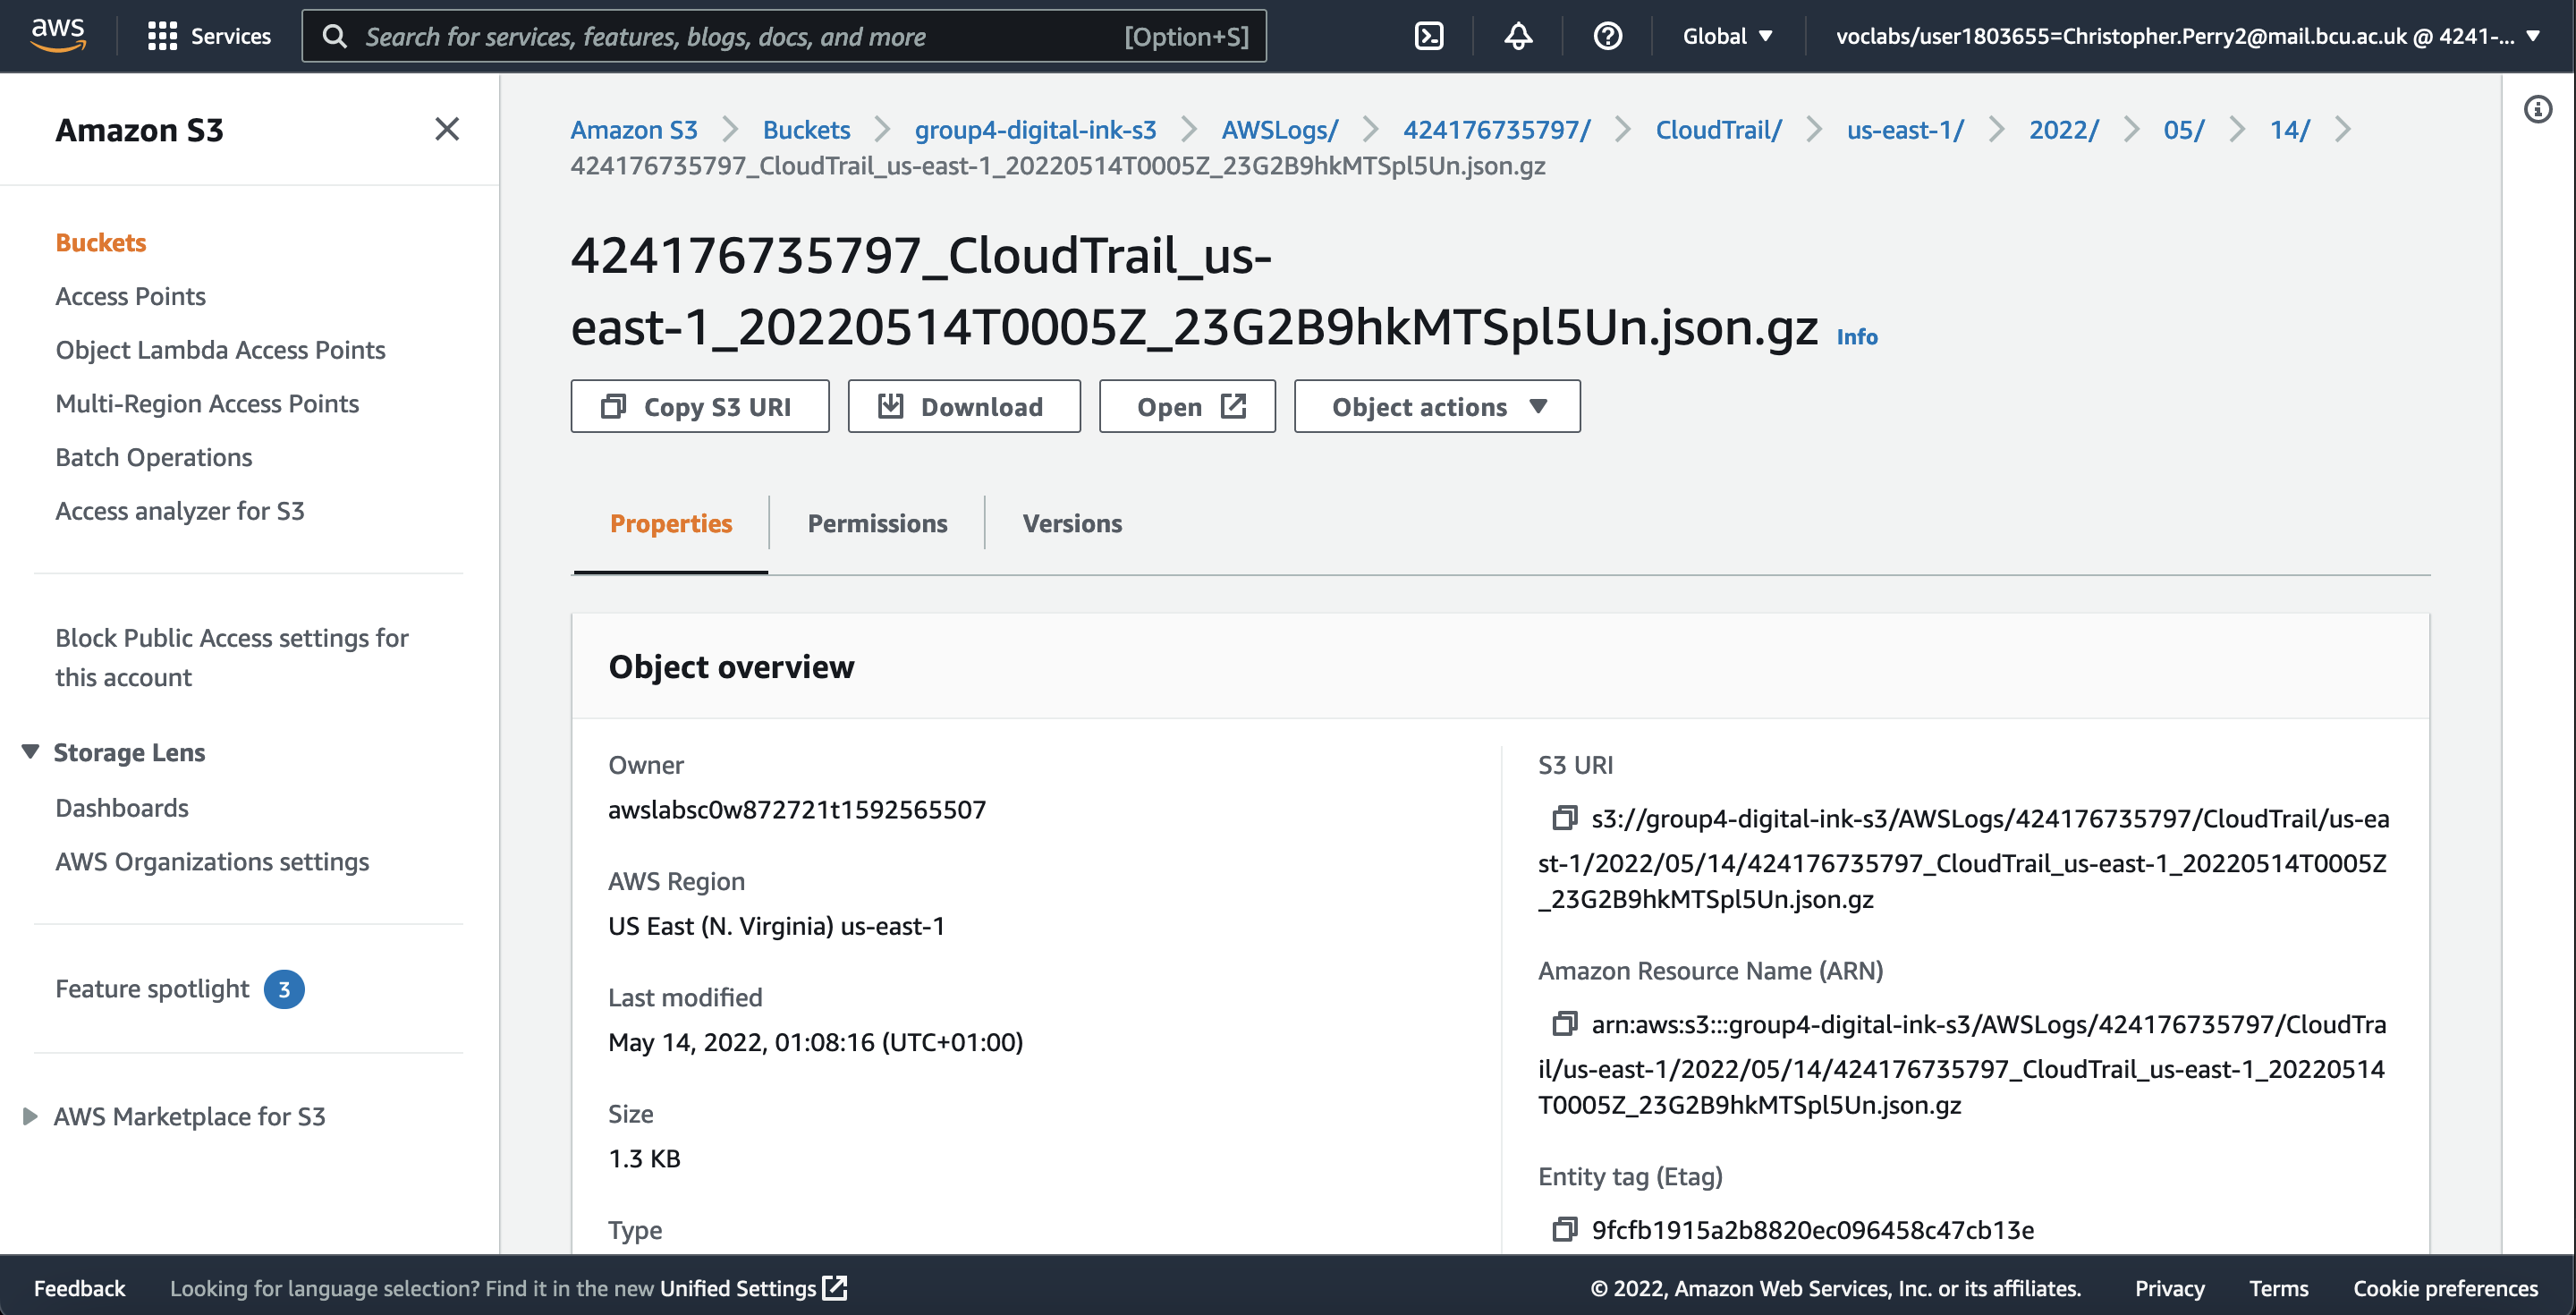
\includegraphics[width=\textwidth]{resources/cloudtrail/cloudtrail-test}
    \caption{CloudTrail test.}
    \label{fig:cloudtrail-test-photo}
\end{figure}

\clearpage
\section{Testing ELB}\label{sec:testing-elb}

\begin{figure}[!htbp]
    \centering
    \begin{minted}{cucumber}
Scenario: Load Balanancer redirect from Instance 1 to Instance 2
    Given that the Group4-Load-Balancer service is active
    When Group4-EC2 is shut down
    Then traffic should be moved to Group4-EC2-Instance-2
    \end{minted}
    \label{fig:elb-test}
\end{figure}

\begin{figure}[!htbp]
    \centering
    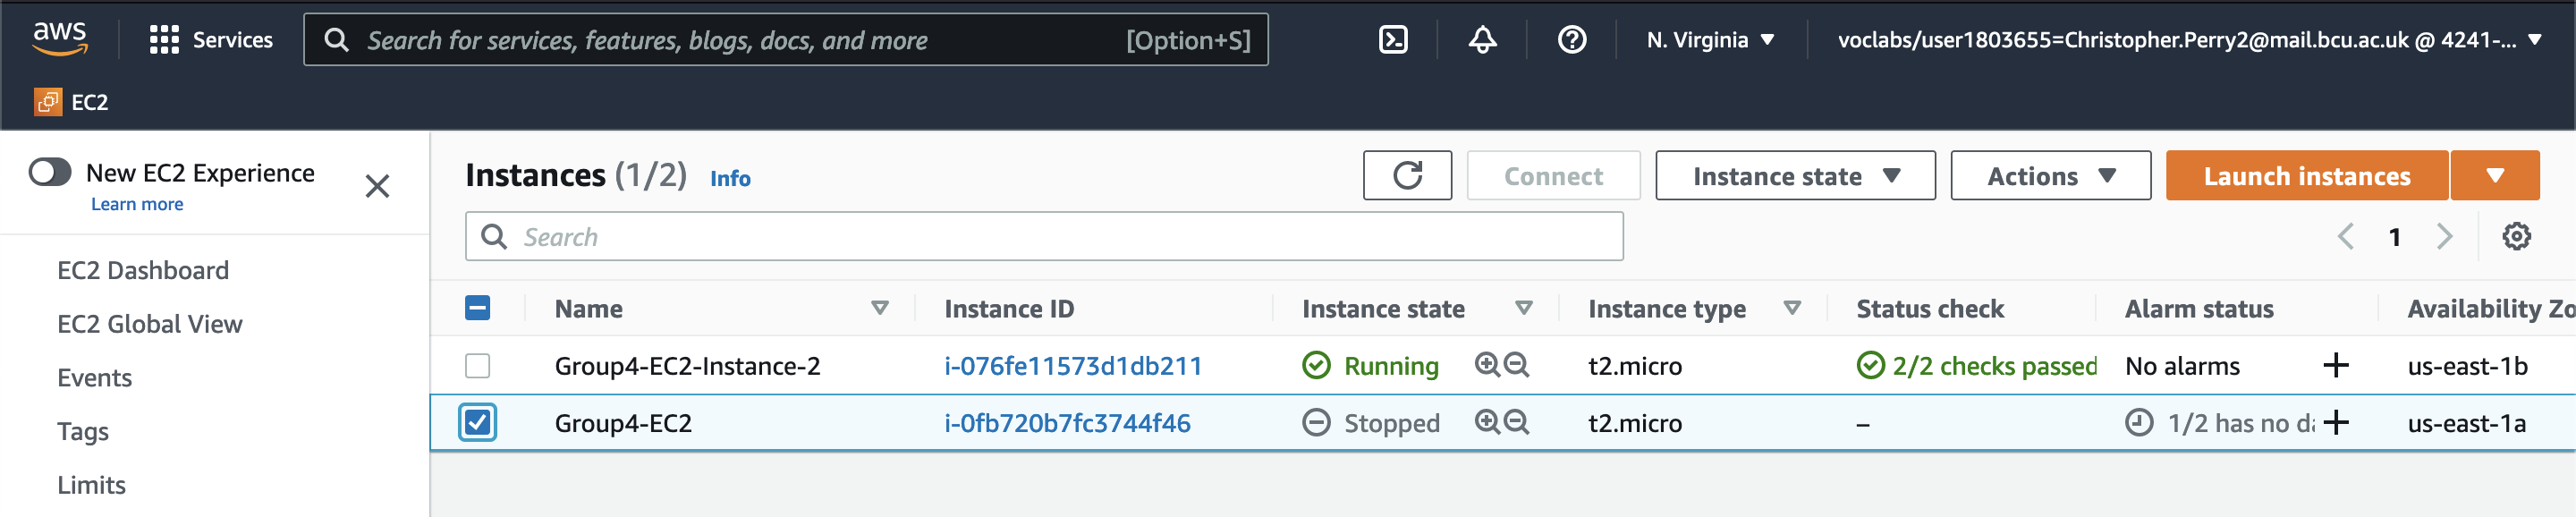
\includegraphics[width=\textwidth]{resources/elb/elb-test-stopped-instance}
    \caption{Stopped Group4-EC2 instance.}
    \label{fig:elb-test-stopped-instance}
\end{figure}

\begin{figure}[!htbp]
    \centering
    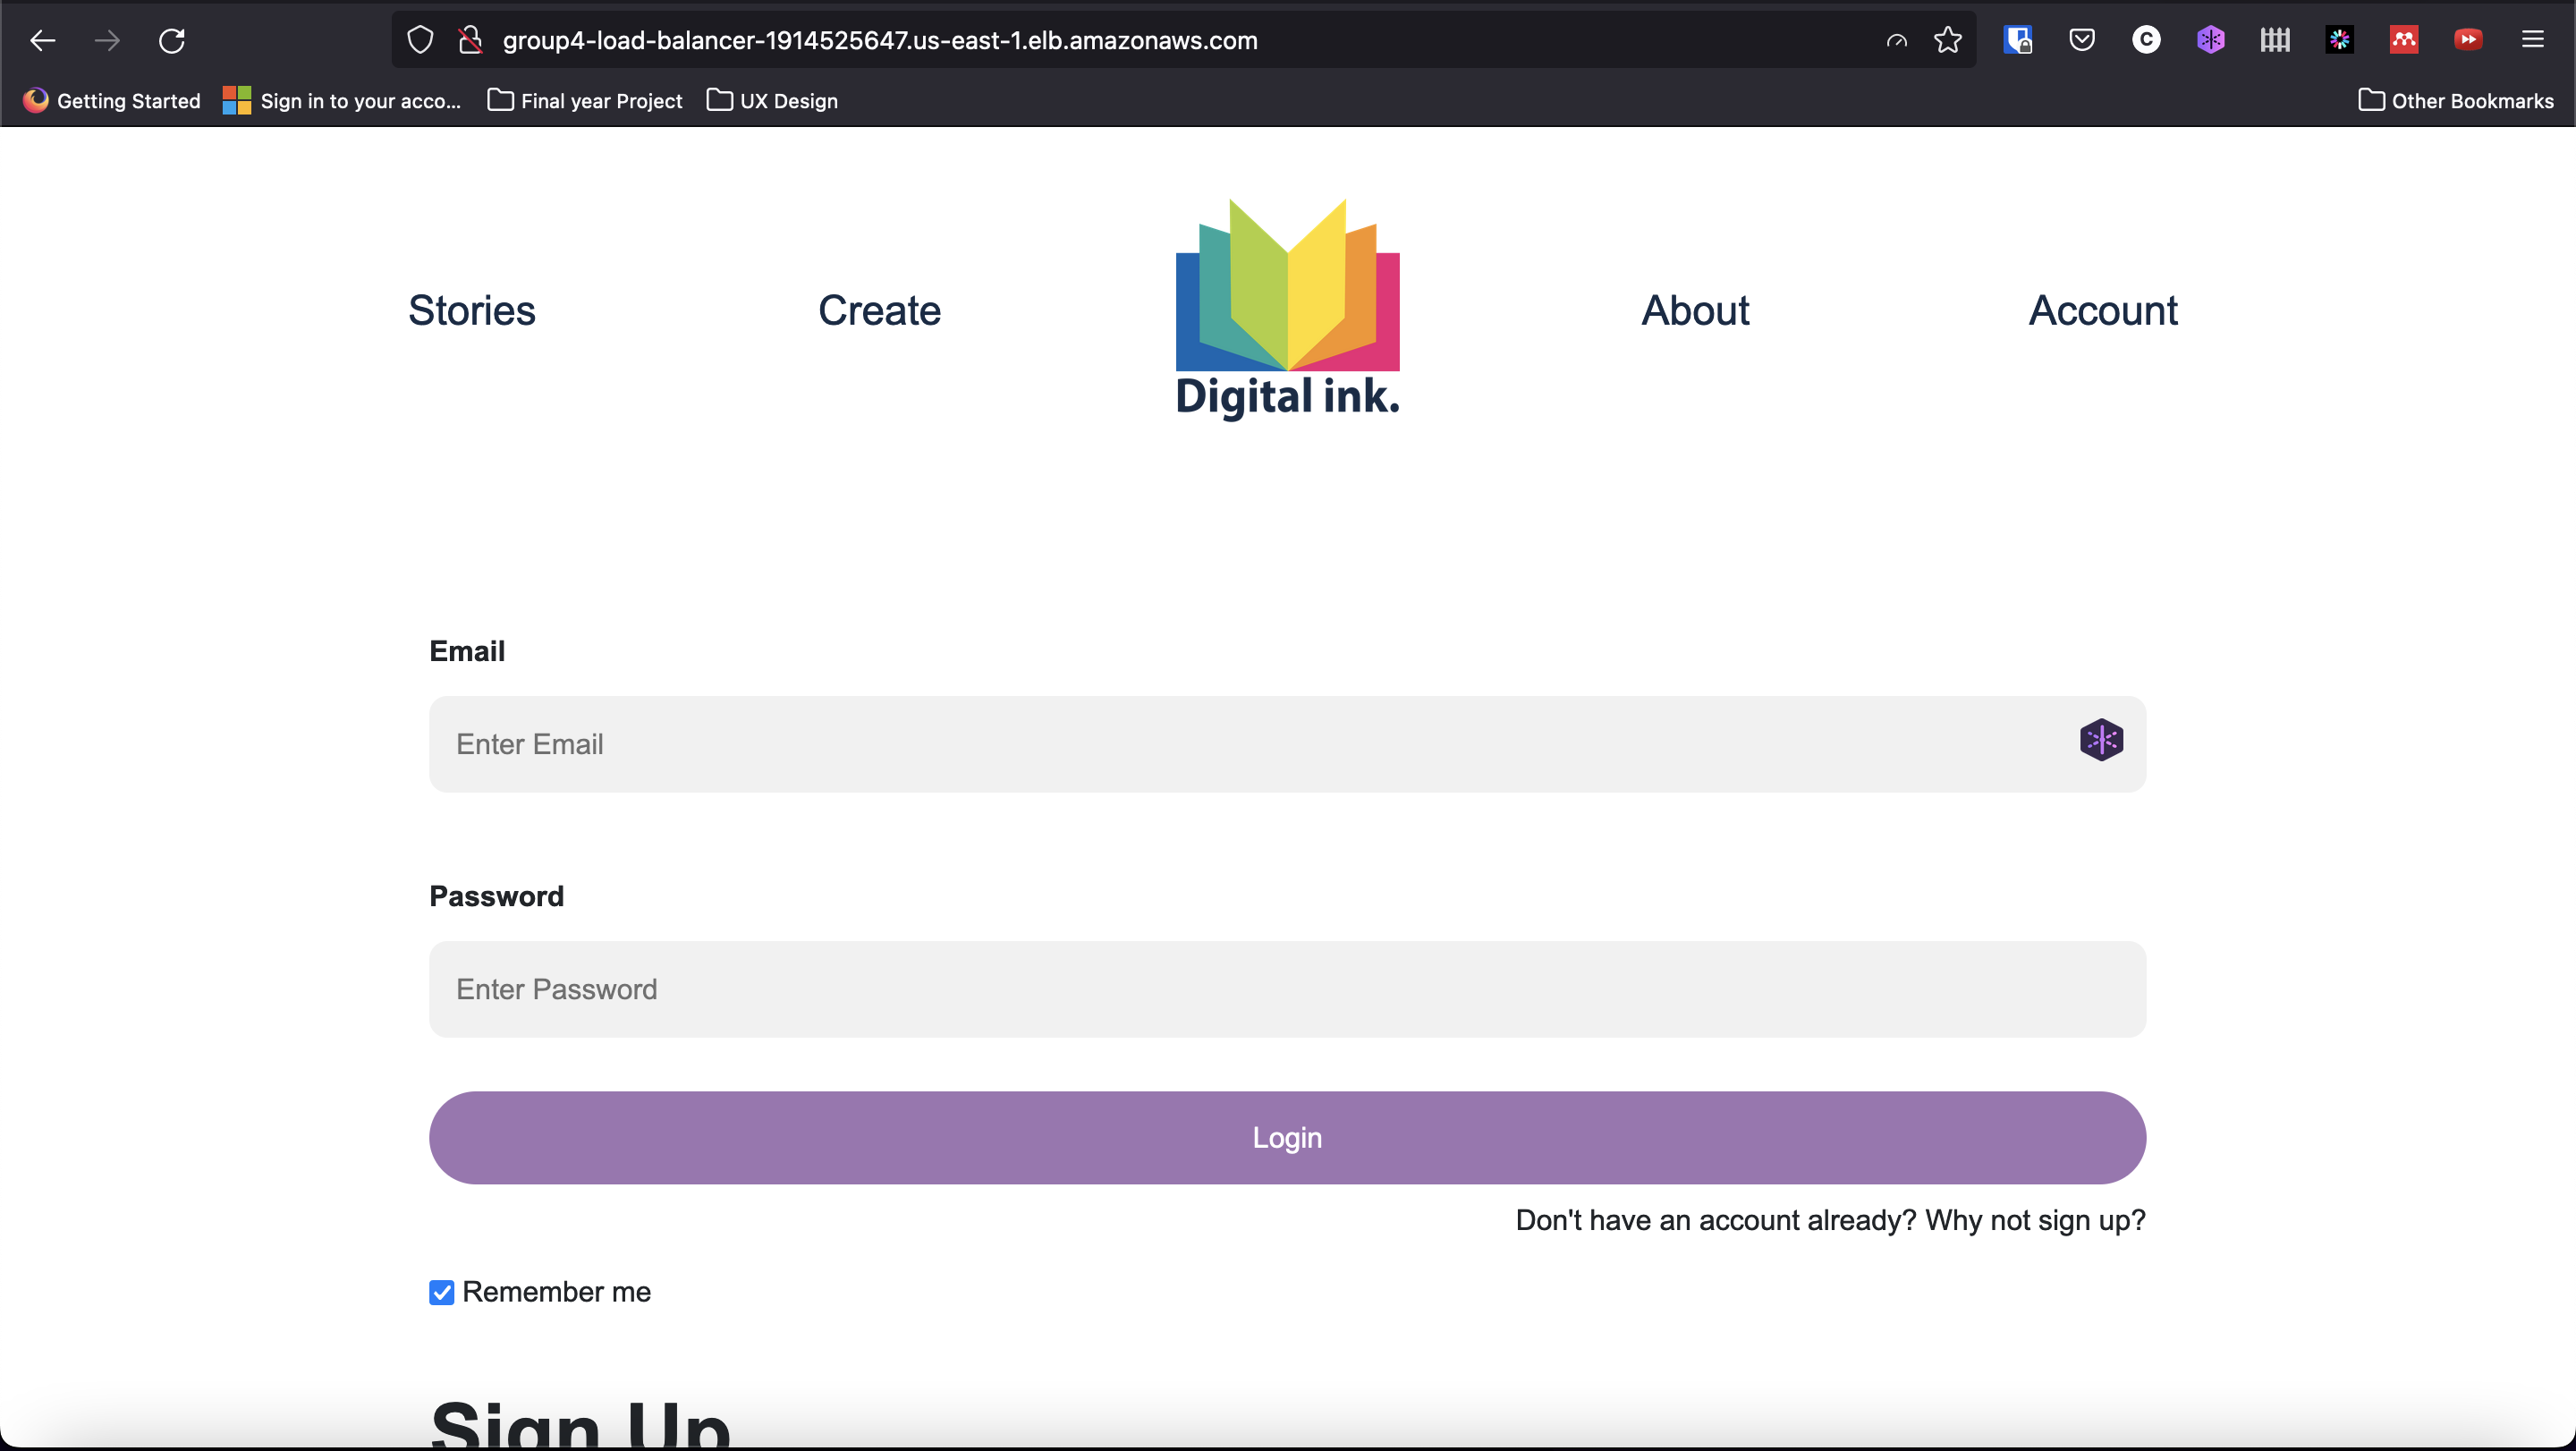
\includegraphics[width=\textwidth]{resources/elb/elb-working}
    \caption{Web app page still loading through other EC2 instance.}
    \label{fig:elb-test-working}
\end{figure}

\clearpage

\begin{figure}[!htbp]
    \centering
    \begin{minted}{cucumber}
Scenario: Load Balanancer redirect from Instance 2 to Instance 1
    Given that the Group4-Load-Balancer service is active
    When Group4-EC2-Instance-2 is shut down
    Then traffic should be moved to Group4-EC2
    \end{minted}
    \label{fig:elb-test-2}
\end{figure}

\begin{figure}[!htbp]
    \centering
    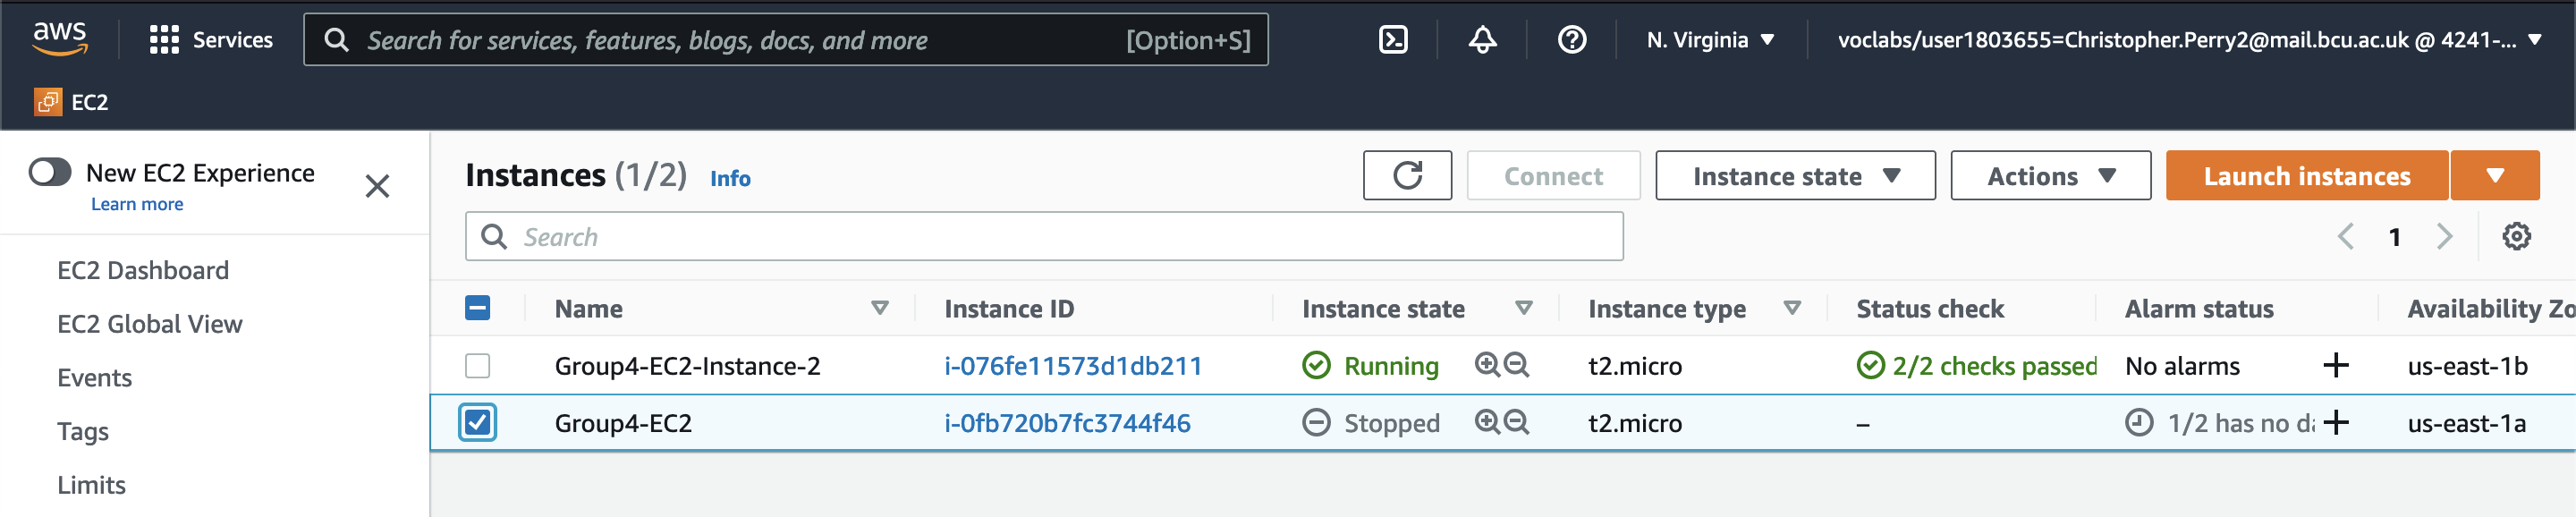
\includegraphics[width=\textwidth]{resources/elb/elb-test-stopped-instance}
    \caption{Stopped Group4-EC2-Instance-2 instance.}
    \label{fig:elb-test-stopped-instance-2}
\end{figure}

\begin{figure}[!htbp]
    \centering
    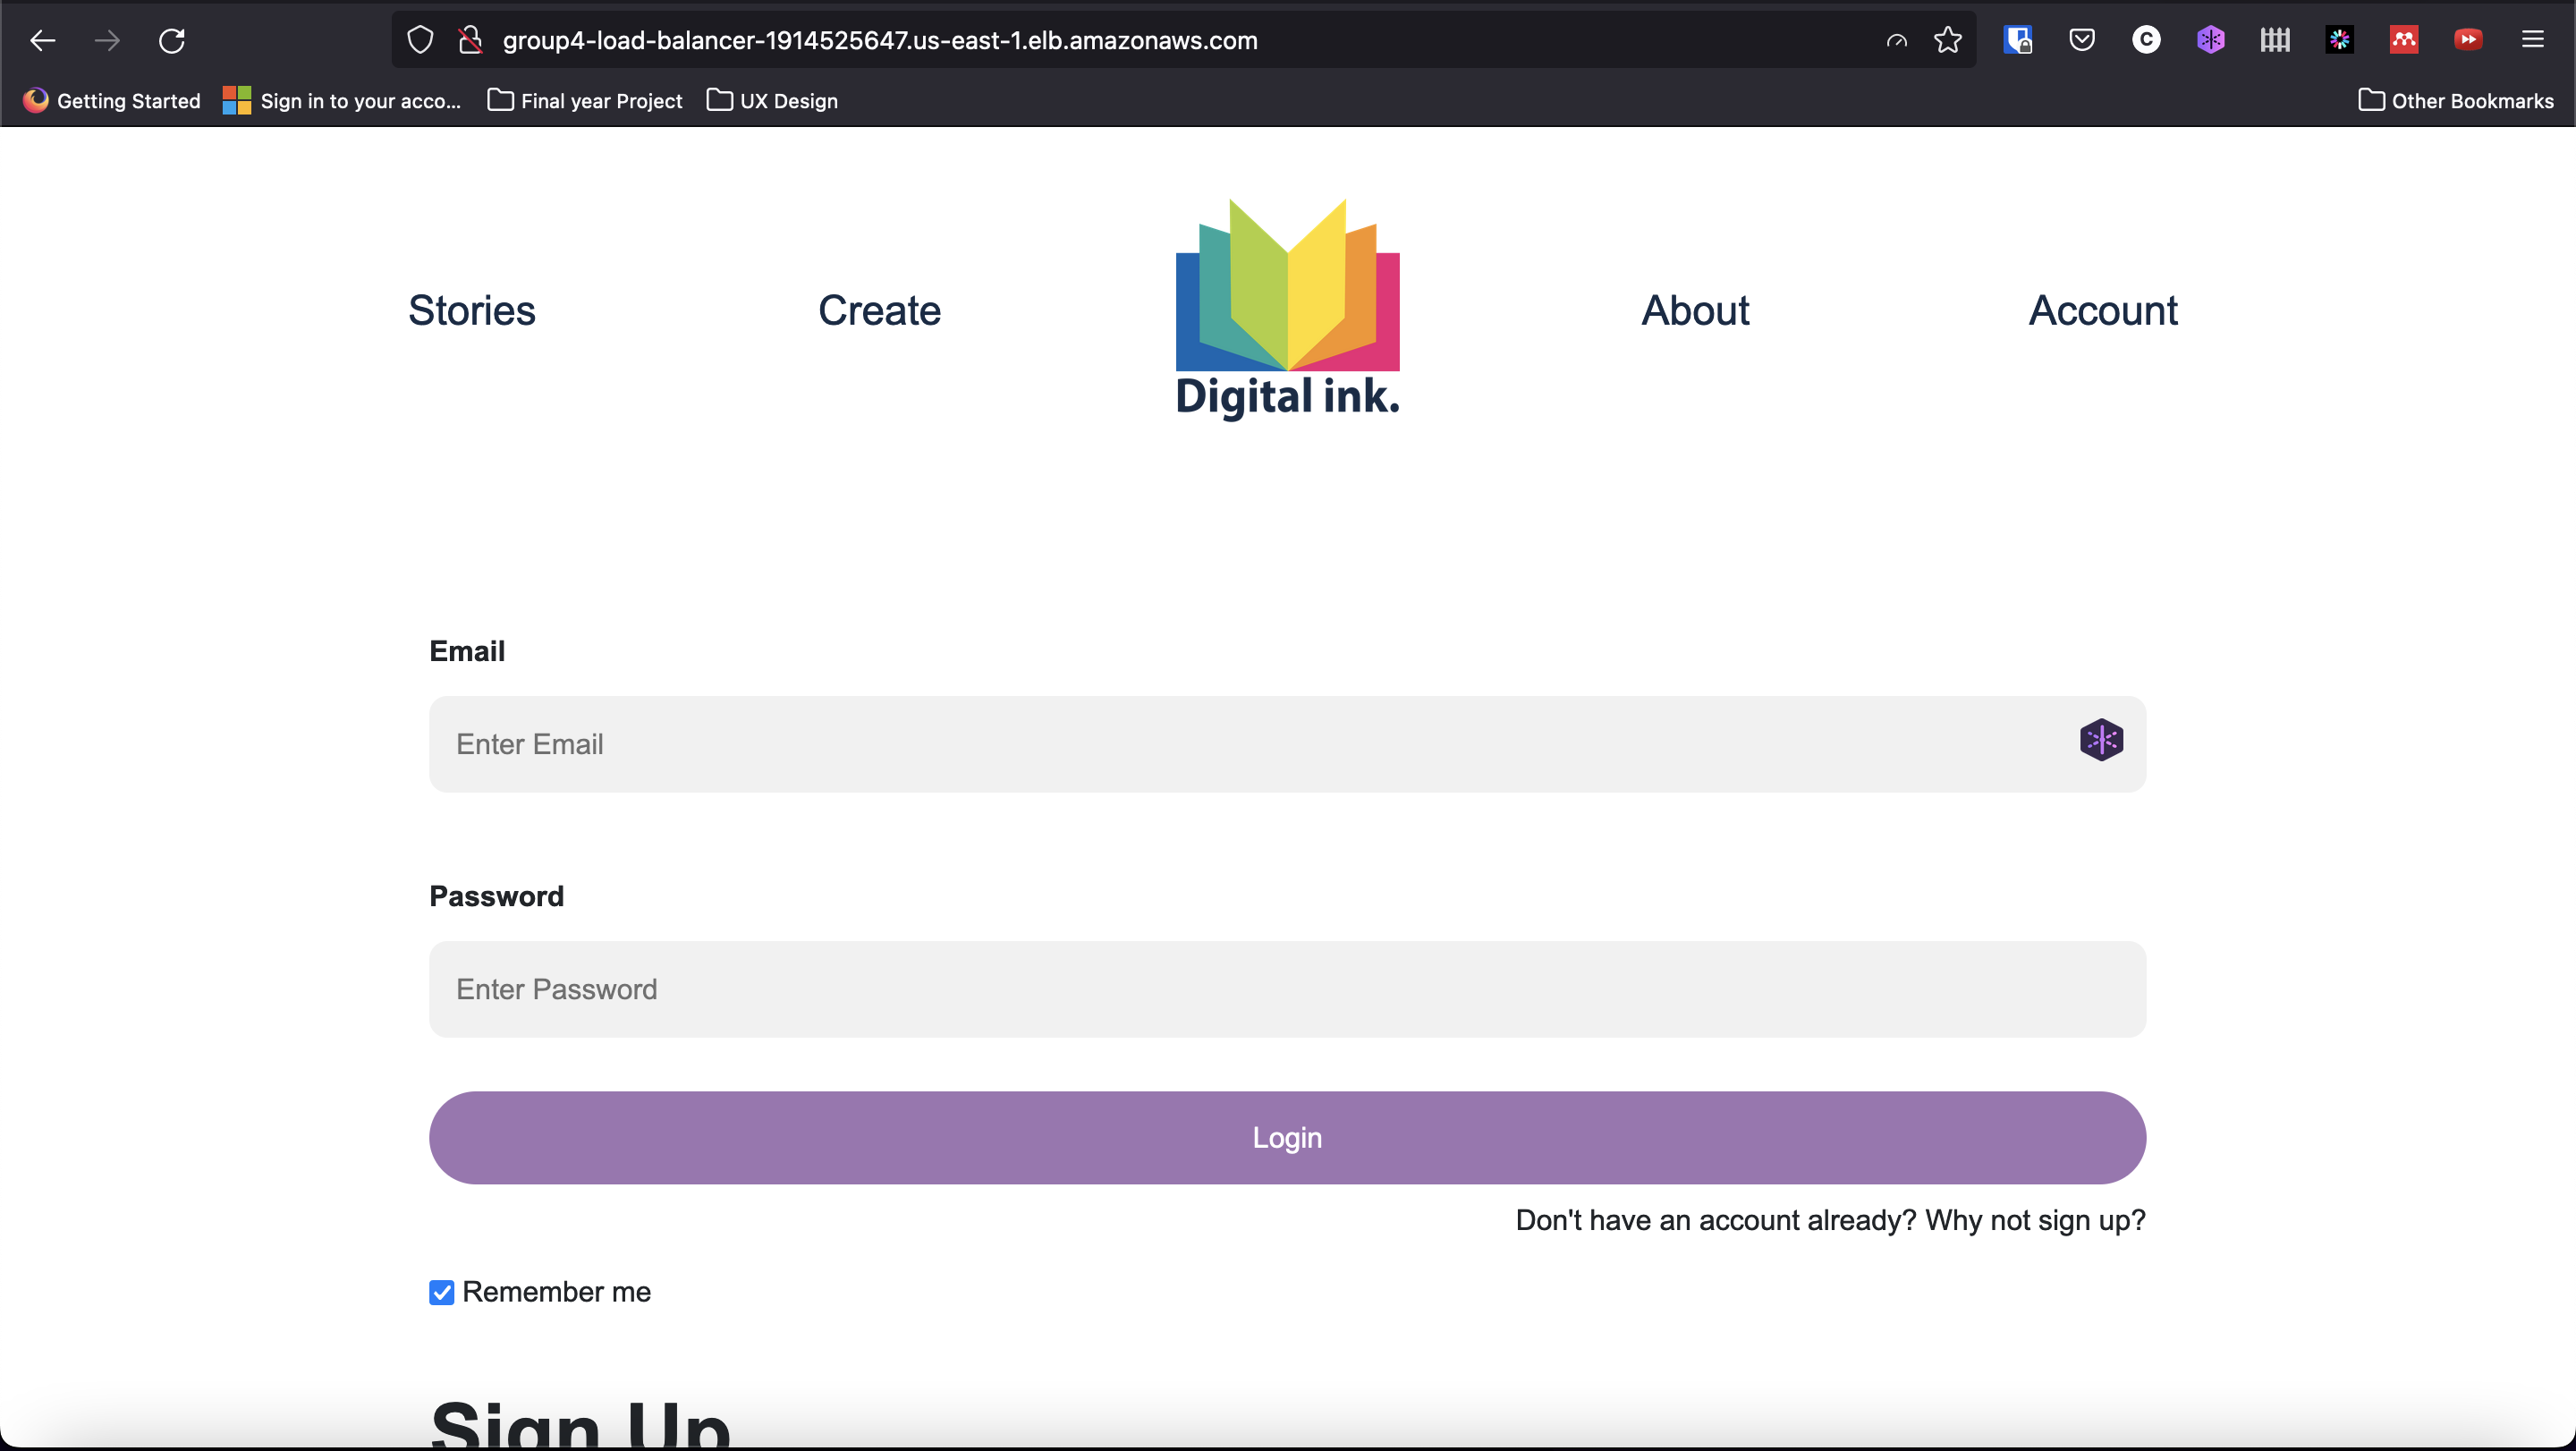
\includegraphics[width=\textwidth]{resources/elb/elb-working}
    \caption{Web app page still loading through other EC2 instance.}
    \label{fig:elb-test-working-2}
\end{figure}



